\documentclass{LU}

\title{Latvijas Padziļināto digitālo prasmju uzlabošana}	   
\thesistype{Maģistra darbs}
\author{Jānis Knets}
\studentid{jk07108}
\supervisor{lektore, M.biz.vad. Daiga Āboltiņa}
\university{Latvijas Universitāte}
\faculty{Biznesa, vadības un ekonomikas fakultāte}
\location{Rīga}

% \pgfplotsset{compat=1.15}

\makeglossaries

\newglossaryentry{agile}
{
    name=Spējā metodoloģija,
    description={Darba organizēšanas metode, kura tiek plaši pielietota IT industrijā}
}

\newacronym{es}{ES}{Eiropas Savienība}
\newacronym{desi}{DESI}{Digital Ekonomikas un Sabiedrības Indekss}

\newacronym{pv}{PV}{kopējā tagadnes vērtība}
\newacronym{npv}{NPV}{tīrā tagadnes vērtība}
\newacronym{irr}{IRR}{iekšējās peļņas norma}
\newacronym{roi}{ROI}{investīciju rentabilitāte}
\newacronym{pi}{PI}{rentabilitātes indekss}
\newacronym{cf}{CF}{tīrā naudas plūsma}
\newacronym{ic}{IC}{projekta investīcijas}
\newacronym{icc}{ICC}{uzkrājošā naudas plūsma}


\begin{document}

\maketitle
\pagenumbering{arabic} % sākam numurēt lapas no apzīmējumu saraksta (3. pielikums iekš LU 03.02.2012, 1/38 ) 

\begin{abstract}
    This document is example on how to use latex and \textit{lu.cls} classs.
\end{abstract}
\selectlanguage{english}
\begin{abstract}
This document is example on how to use latex and \textit{lu.cls} classs.
\end{abstract}
\selectlanguage{latvian}
\setcounter{page}{3}
\tableofcontents

%------------------------------------------------APZĪMĒJUMI---------------------------------------------------------

\pagestyle{plain}
\printglossary[title=Termini, toctitle=Termini]
\printglossary[type=\acronymtype,title=Akronīmi, toctitle=Akronīmi]
\chapter*{Ievads} % * asterisk does not number the chapter
\addcontentsline{toc}{chapter}{Ievads} %adds unnumbered section to table of contents
Dotā maģistra darba aktualitāti nosaka ta, ka Latvijā jau vairākus gadus ir izjūtams darbinieku 
trūkums IT nozarē. Otrs ietkmējošais faktors ir tas, ka digitālās tehnoloģijas ar vien vairāk
ienāk mūsu ikdienas dzīvē, tās ir jāizmanto ar vien plašākā darba vietu skaitā; Taču Latvijā
digitālo prasmju līmenis ir salīdzinoši zems. 
\par
Dotajā darbā autors cenšas risināt šīs problēmas ar Start(it) fonda pieejamiem resursiem. Fonda mērķis
ir popularizēt datoriku Latvijas skolās. Šī fonda eksistējošā vietne tiks uzlabota tā, lai varētu 
nodrošināt apmācības plašākam cilvēku lokam.
\par
Projekta \textbf{pētījuma objekts} ir digitālās prasmes Latvijā.
\textbf{Maģistra darba mērķis} ir padziļināto digitālo prasmju apmācību paplašināšanas iespējas Latvijā.

\par
\textbf{Mērķa sasniegšanai veicamie uzdevumi} ietver:
\begin{enumerate}
    \item nozares raksturojuma veikšanu, noskaidrojot aktuālās tendences;
    \item noskaidrot nozares ekspertu viedokli par padziļinātām datorprasmēm, to pieejamību un nozīmīgumu;
    \item veikt problēmas noteikšanu un analīzi;
    \item izstrādāt projekta priekšlikumu;
    \item izstrādāt projekta īstenošanas rokasgrāmatu;
    \item izstrādāt secinājumus un priekšlikumus.
\end{enumerate}
\par
Maģistra darbu veido trīs daļas, kā arī secinājumi, priekšlikumi un pielikumi.
Darba \textbf{pirmajā nodaļā} tiek aplūkots Eiropas Savienības \acrshort{desi} indekss, kurš norāda
cik labi ir ieviestas digitālās inovācijas Eiropas valstīs un tās tiek savstarpēji salīdzinātas. Turpmāk
tiek apskatīti Latvijā eksistējošo kursu piedāvājumi un Skola 2030 apraksts. Tiek veikta digitālo prasmju
nozīmīguma un kursu pieejamības analīze ekspertu skatījumā. Šīs analīzes rezultātā tiek izvirzīta 
pamatproblēma, veikta tās analīze un izvēlēta konkrēti risināmā problēma. 
\textbf{Otrajā nodaļā} tiek definēti projekta mērķi, turpinājumā tiek izvirzītas trīs projekta alternatīvas,
Šīs alternatīvas tiek izvērtētas pēc dažādiem kritērijiem. Otrā nodaļas beigās tiek izvēlēta labākā alternatīva, 
kura tiek noformēta projekta priekšlikuma veidā. 
\textbf{Trešajā nodaļā} tiek izveidota projekta rokasgrāmata iepriekšējā nodaļā izvēlētajai alternatīvai,
kurā ietverts projekta starts, plānošana, pamatkoncepcija, detaļkoncepcija, realizācija, ieviešana un noslēgums. 
Darba noslēgumā tiek piedāvāti autora secinājumi un priekšlikumi.
\par
\textbf{Pētniecības metodes}, kuras autors izmantojis ir datu analīze,
prāta kartes, intervijas, riksa analīzes, tīkla plānošanu
\par
\textbf{Pētījuma periods} no 2005 līdz 2019
\par
Maģistra darba izstrādes procesa tika izmantoti tādi \textbf{literatūras un datu avoti} kā statistikas dati
gan no Eiropas Savienības, gan arī Latvijas, zinātniiskie darbi, noslēguma darbi, publiski pieejamā informācija
no tīmekļa vietnēm, projektu vadības teorijas literatūra un citi materiāli.

\chapter{Digitālo prasmju ietekmes analīze uz darba tirgu}
\paragraph{}
Mūsdienu pasaule strauj attīstās un ar vien vairāk tiek runātas par dažādu arodu izzušanu.
Taču veidojās arī jaunie darba veidi, ar vien vairāk šie jaunie arodi prasa cilvēkam zināt
jaunās tehnoloģijas, datorprasmi gan pamatprasmju līmenī, gan padziļināti.
Autors veic izpēti par Latvijas rādītājiem Eiropas Savienības līmenī izmantojot \acrlong{desi} 
(turpmāk tekstā \acrshort{desi}), kā arī šie rādītāji ir salīdzināti ar Latvijas tuvākiem kaimiņiem,
proti, Lietuvu un Igauniju.Otra datu grupa nāk no Latvijas atvērtās datu kopas, pievēršot plašāku 
uzmanību izglītībai un nodarbinātībai ITK jomai. Šī datu izpēte nepieciešama, lai varētu pieņemt 
labāku lēmumu par uzņēmuma Accenture Latvijas filiāle turpmāko sadarbību izglītības sektorā.
\paragraph{}
Accenture Latvia par savu korperatīvo sociālo atbildību ir izvirzījusi tieši attīstību. Tam par pamatu nāk lielā nepieciešamība
pēc augsti kvalificētā darba spēka. Uzņēmums jau vairāk nekā 15 gadus veiksmīgi darbojas Latvijas teritorijā, taču asi izjūt
darba spēka trūkumu. Ieguldījums izglītībā palīdz labot situāciju, kā arī uzlabo Latvijas kopējo konkurētspēju Eiropā un pasaulē.
\section{Digitālās ekonomikas un savienojamības indeks}
%example plot
\textit{The \LaTeX\ Companion} book \cite{latexcompanion}
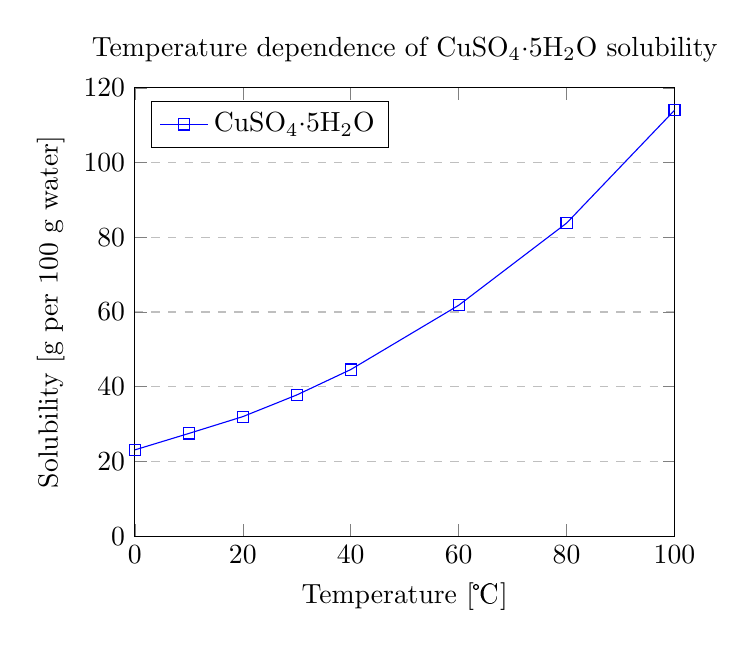
\begin{tikzpicture}
    \begin{axis}[
        title={Temperature dependence of CuSO$_4\cdot$5H$_2$O solubility},
        xlabel={Temperature [\textcelsius]},
        ylabel={Solubility [g per 100 g water]},
        xmin=0, xmax=100,
        ymin=0, ymax=120,
        xtick={0,20,40,60,80,100},
        ytick={0,20,40,60,80,100,120},
        legend pos=north west,
        ymajorgrids=true,
        grid style=dashed,
    ]
     
    \addplot[
        color=blue,
        mark=square,
        ]
        coordinates {
        (0,23.1)(10,27.5)(20,32)(30,37.8)(40,44.6)(60,61.8)(80,83.8)(100,114)
        };
        \legend{CuSO$_4\cdot$5H$_2$O}
     
    \end{axis}
\end{tikzpicture}
    \subsection{Savienojamība}
\begin{figure}[h]
    \label{att:desi_savienojamiba}
    \caption{DESI rādītāji}
    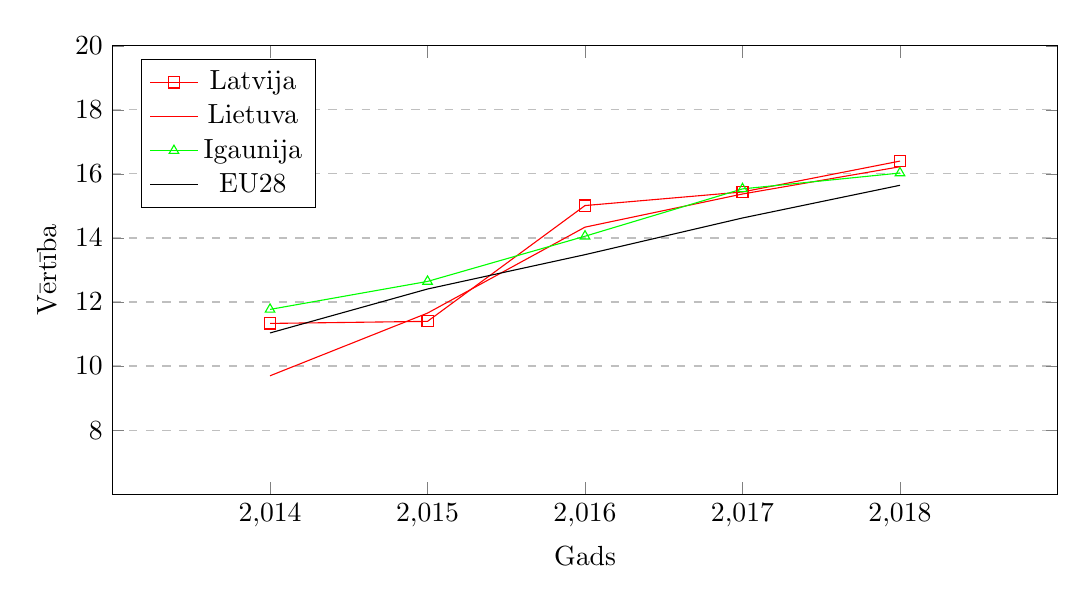
\begin{tikzpicture}
        \begin{axis}[
            x=2cm,
            xlabel={Gads},
            ylabel={Vērtība},
            xmin=2013, xmax=2019,
            ymin=6, ymax=20,
            xtick={2014,2015,2016,2017,2018},
            ytick={8,10,12,14,16,18,20},
            legend pos=north west,
            ymajorgrids=true,
            grid style=dashed,
        ]
        \addplot[
            color=red, 
            mark=square
            ]
            coordinates {
                (2014,11.3305)(2015,11.3951)(2016,15.0115)(2017,15.4357)(2018,16.4)
            };
        \addplot[
            color=red, 
            mark=circle
            ]
            coordinates {
                (2014,9.6959)(2015,11.6532)(2016,14.3374)(2017,15.3726)(2018,16.2237)
            };
        \addplot[
            color=green, 
            mark=triangle
            ]
            coordinates {
                (2014,11.7685)(2015,12.6421)(2016,14.0537)(2017,15.5321)(2018,16.0279)
            };
        \addplot[
            color=black, 
            mark=dot
            ]
            coordinates {
                (2014,11.0332)(2015,12.4053)(2016,13.478)(2017,14.6234)(2018,15.6445)
            };
        \legend{Latvija, Lietuva, Igaunija, EU28}
        \end{axis}
    \end{tikzpicture}
\end{figure}
\paragraph{}
2017. gadā Latvijai izdevās panākt diezgan lielu progresu kopējā savienojamības
aspektā, un tās izaugsmes temps līdzinājās ES vidējam. Attiecībā uz mājsaimniecību
fiksētās platjoslas pārklājumu valstī vērojama stagnācija – tā joprojām atpaliek no ES
vidējā rādītāja, ar 93\% mājsaimniecību pārklājumu Latvijai atrodoties 24. vietā.
Jāuzsver, ka gandrīz viss pārklājums nodrošina nākamās paaudzes piekļuvi (NPP)
(91\% mājsaimniecību) un pat ātrdarbīgo platjoslu (88\% mājsaimniecību), tādējādi
Latviju ierindojot starp vadošajām dalībvalstīm, kuru rādītāji krietni pārsniedz ES
vidējo. Arī 4G pārklājums Latvijā ir ļoti augsts (98\% mājsaimniecību). Ātrdarbīgās un
īpaši ātrdarbīgās platjoslas izmantošanas līmenis arī ir ievērojami augstāks par ES
vidējo: 42\% un 35\% mājokļu abonē ātrdarbīgas un īpaši ātrdarbīgas platjoslas
pakalpojumus, kas attiecīgi Eiropas Savienībā vidēji ir 33\% un 15,4\%. Tomēr,
neskatoties uz nelielu pieaugumu 2017. gadā, kopējā fiksētās platjoslas izmantošana
Latvijā vēl aizvien ir mazliet zem ES vidējā rādītāja. Šo tendenci zināmā mērā 
Digitālās ekonomikas un sabiedrības indekss 2018, ziņojums par Latviju. lpp. 4 no 11
kompensē daudz straujākais mobilās platjoslas pieslēgumu pieaugums, jo ir plašas
iespējas izvēlēties datu plānus par pieejamām cenām.
\paragraph{}
“Vidējās jūdzes projekts”, kas tika sākts 2012. gadā un kam piešķirts līdzfinansējums
no ES struktūrfondiem, lai lauku teritorijas savienotu ar valsts pamatinfrastruktūru,
tagad nonācis otrajā posmā. Plānots, ka otrā posma būvdarbi sāksies 2018. gada
pavasarī. Galvenokārt tie tiks veikti atlikušajās “baltajās” teritorijās (2014.–2015. gadā
apzināta 221 teritorija). Paredzēts, ka līdz 2020. gadam optiskie kabeļi tiks ierīkoti
2800 km garumā un izveidoti aptuveni 220 optiskā tīkla piekļuves punkti. Pēc tam
telesakaru operatoriem, izmantojot jauno tīklu, kas ļaus galalietotājiem piedāvāt
mazumtirdzniecības pakalpojumus, būs iespēja izveidot vietējās sakaru līnijas ar datu
pārraides ātrumu vismaz 30 Mbit/s (“pēdējā jūdze”). Tomēr šķiet, ka ne visur tiek
veiktas privātās investīcijas “pēdējās jūdzes” infrastruktūras izbūvē. Ir vajadzīgi
turpmāki centieni, piemēram, papildu valsts atbalsta shēmas un regulatīvi pasākumi,
lai novērtētu situāciju un piedāvātu risinājumus, kas attiecīgajos gadījumos ļautu
novērst ar “pēdējo jūdzi” saistīto plaisu. Iespēja mājās, pieslēdzoties no mobilajām
ierīcēm, izmantot mobilo operatoru nodrošinātos fiksētos sakaru pakalpojumus,
palīdz pārvarēt šo plaisu atsevišķos lauku apvidos, kur netiek veiktas investīcijas
“pēdējās jūdzes” savienojumos\cite{platjosla}
\paragraph{}
Optiskā tīkla izveidē un 4G pakalpojumu ieviešanā Latvija ir izvirzījusies starp
līderiem. Tomēr joprojām problemātiska ir digitālā plaisa, kas izveidojusies starp
pilsētu un laukiem. Lai to novērstu, praktisku labumu var sniegt nesen pieņemtie
noteikumi, ar kuriem tiek transponēta Platjoslas izmaksu samazināšanas direktīva.
Turklāt, lai nākotnē neatpaliktu no straujās savienojamības attīstības, visiem tirgus
dalībniekiem jābūt savlaicīgi pieejamiem piemērotiem spektra blokiem agrīnai 5G
tīkla izmēģināšanai un izvēršanai.

    \paragraph{}
Cilvēkkapitāla aspektā Latvija atpaliek no ES vidējās vērtības, un pēdējā gadā progress nav
panākts. Interneta lietotāju īpatsvars iedzīvotāju vidū gandrīz atbilst ES vidējam rādītājam,
tomēr 52 \% Latvijas iedzīvotāju joprojām trūkst digitālo pamatprasmju, kas tiem liedz efektīvi
lietot internetu, turklāt 19 \% digitālo prasmju vispār nav (par 2 punktiem vairāk nekā ES
vidējais rādītājs).
\paragraph{}
Latvijā digitālo prasmju līmenis sieviešu vidū ir nedaudz augstāks nekā vīriešiem. Sieviešu
vidū vismaz 50 \% ir digitālās pamatprasmes, taču vīriešiem tie ir tikai 46 \%. Atšķirīgs ir arī
strādājošo un nestrādājošo iedzīvotāju digitālo prasmju līmenis. No strādājošajiem 57 \%
digitālās prasmes ir pamata vai augstākā līmenī, savukārt nestrādājošo vidū šis rādītājs ir
tikai 33 \%. Arī izglītības līmenis ir svarīgs faktors saistībā ar digitālo prasmju apguvi. No tiem,
kas ieguvuši augstāko izglītību, 76 \% ir vismaz digitālās pamatprasmes (ES līmenī tie ir
84 \%), taču pamatizglītību vai vidēja līmeņa izglītību ieguvušo vidū šis īpatsvars ir tikai 35 \%.
Mazizglītotiem cilvēkiem šis rādītājs ir par 5 \% augstāks nekā ES vidējais, savukārt vidēji
izglītotiem cilvēkiem šī starpība salīdzinājumā ar ES vidējo rādītāju ir 20 punkti. IKT
speciālistu skaits ir stabils, taču ievērojami zem ES vidējā līmeņa. Turklāt pēdējos gados ir
samazinājies absolventu skaits STEM jomā (2013. gadā 14,1, bet 2016. gadā tikai 12,7 uz
1000 iedzīvotājiem).
\paragraph{}
Izglītības attīstības pamatnostādnes 2014.–2020. gadam ietver rīcības virzienus, kas skar
IKT izmantošanu mācību procesā un digitālo prasmju pilnveidošanu. Dokumentā
“Informācijas sabiedrības attīstības pamatnostādnes 2014.–2020. gadam” zem pīlāra “IKT
izglītība un e-prasmes” ir paredzētas šādas darbības izglītības jomā: sabiedrības informētība
Indeksā DESI 2018 izmantoti jaunākie dati. Tie var būt 2015. vai 2016. gada dati, atkarībā no konkrētās
dalībvalsts. Tas atspoguļojas DESI 2018. gada sarindojumā. Eurostat ir koriģējis vēsturiskos datus.
Digitālās ekonomikas un sabiedrības indekss 2018, ziņojums par Latviju. lpp. 6 no 11
un gatavība izmantot e-iespējas, iedzīvotāju un uzņēmēju e-prasmju pilnveidošana, IKT
prasmju palielināšana valsts pārvaldē, IKT speciālistu un darbinieku sagatavošana atbilstīgi
darba tirgus vajadzībām, kā arī algoritmiskās domāšanas un informācijpratības palielināšana
izglītības programmās. Šīm darbībām tiek piešķirts valsts finansējums, kā arī ES finanšu
atbalsts.
\paragraph{}
Turklāt Latvijā ir izveidota sava digitālo prasmju un darbvietu koalīcija, kurā iesaistītas
vairākas ministrijas, IKT nozares apvienības un uzņēmumi, kā arī Latvijas Tirdzniecības un
rūpniecības kamera. Koalīcijas darbu koordinē Latvijas Informācijas un komunikācijas
tehnoloģijas asociācija (LIKTA). Koalīcijas darbā ir noteikti prioritārie virzieni, kas definēti
iepriekš minētajos dokumentos un kas orientēti uz šādiem mērķiem: nodrošināt IKT
apmācību atbilstīgi darba tirgus vajadzībām, iesaistīt jauniešus IKT jomā, izveidot
mūsdienīgus un interaktīvus mācību procesus, palielināt informētību par digitālās pratības un
IKT prasmju nozīmīgumu.
\paragraph{}
Pagājušajā gadā ir veikti vairāki pasākumi, lai īstenotu šīs stratēģijas, piemēram, projekti
“MVU apmācības inovāciju un digitālo tehnoloģiju attīstībai Latvijā” un “IKT profesionāļu
apmācības inovāciju veicināšanai un nozares attīstībai”. Šo projektu mērķis: sniedzot
iespēju apgūt nākotnes digitālajās darbvietās vajadzīgās IKT prasmes, atbalstīt jauniešu
nodarbināmību un personisko izaugsmi. Mērķis ir laikposmā no 2017. līdz 2020. gadam
noorganizēt augstas kvalitātes digitālo prasmju kursus 7000 MVU darbiniekiem un 1500 IKT
speciālistiem. 2017. gada oktobra beigās pirmajā projektā bija iesaistījušies jau vairāk nekā
400 uzņēmumi un no 7000 iecerētajām apmācībām bija noorganizētas vairāk nekā 900. Ap
šo pašu laiku 55 IKT uzņēmumi bija iesaistījušies otrajā projektā un 196 augsta līmeņa
specializētos IKT apmācību kursos savas prasmes un kvalifikācijas bija atjauninājuši 780 IKT
speciālistu.
\paragraph{}
Šajā jomā ir veikti daudzsološi pasākumi, un var paiet noteikts laiks, kamēr būs jūtama to
ietekme, taču Latvijai vēl ir jāstrādā pie tā, lai uzlabotu iedzīvotāju un darbaspēka digitālās
prasmes, tādējādi labāk sagatavojoties savas tautsaimniecības un iedzīvotāju digitālajai
pārejai
    \subsection{Interneta lietošana}
Interneta lietotāju īpatsvars Latvijas iedzīvotāju vidū joprojām pārsniedz ES vidējo rādītāju.
Jo īpaši augstāks par vidējo ir internetbankas lietotāju īpatsvars (75 \%, kas Latviju ierindo 8.
vietā ES), taču iecienīti ir arī citi interneta pakalpojumi – ziņu lasīšana (84 \%), mūzikas
klausīšanās, video skatīšanās vai spēļu spēlēšana (77 \%) un sociālo tīklu izmantošana
(74 \%). No otras puses, iepirkšanās tiešsaistē ir salīdzinoši mazāk populāra. Patiešām,
pagājušajā gadā tikai nedaudz vairāk par pusi (55 \%) interneta lietotāju norādīja, ka 2017.
gadā ir iepirkušies tiešsaistē (ES tie ir 68 \%).
    \desigraph{desi_integrācija}{Integrācija}
  {(2014,3.66053)(2015,3.53131)(2016,4.24364)(2017,4.54676)(2018,5.40541)}
  {(2014,7.73173)(2015,7.69844)(2016,8.29504)(2017,8.8177)(2018,9.49093)}
  {(2014,4.33245)(2015,4.72564)(2016,5.35507)(2017,6.3295)(2018,7.4129)}
  {(2014,5.49634)(2015,6.15731)(2016,6.91282)(2017,7.34056)(2018,8.01831)}

  Definīcija - 4a Uzņēmumu digitalizācija (60\%), 4b eKomercija (40\%)
\par

Pagājušajā gadā saistībā ar digitālo tehnoloģiju integrāciju uzņēmumos Latvija ir guvusi
labus panākumus, no 25. vietas 2017. gadā pakāpjoties uz 23. vietu. Tomēr šajā jomā tā
joprojām atpaliek no lielākās daļas ES valstu. Situācijas uzlabošanos ietekmējuši uzņēmumi,
kas iegādājušies mākoņdatošanas pakalpojumus (pagājušajā gadā šis apjoms gandrīz
dubultojies, tagad sasniedzot 9,4 \%), un uzņēmumi, kas pieņēmuši elektronisku informācijas
koplietošanu. Par 2,5 procentpunktiem, sasniedzot 10,6 \%, palielinājies arī to MVU īpatsvars,
kas izmanto elektroniskos pārdošanas kanālus, tādējādi samazinot atšķirību no ES vidējā
rādītāja (17 \%). Nedaudz palielinājies arī to MVU apgrozījums, kuri nodarbojas ar ekomerciju 
(+0,5 procentpunkti, sasniedzot 8,6 \%). Tomēr varētu panākt vēl dažus
uzlabojumus, jo patlaban salīdzinoši maz uzņēmumu nodarbojas ar pārdošanu tiešsaistē pāri
robežām (4,7 \%). Augstās piegādes izmaksas ir galvenais šķērslis, ar ko nākas saskarties
uzņēmumiem, kuri vēlas tiešsaistē pārdot preces klientiem citās ES valstīs.
\par
Latvija nav izstrādājusi visaptverošu stratēģiju uzņēmumu digitalizācijai. Tomēr ir
sagatavotas vairākas iniciatīvas, kas sekmē “Rūpniecība 4.0” (Industry 4.0) izveidi; kā
piemēri minami izmēģinājuma projekts inženiertehniskajā nozarē, kas veicina izpratni par
koncepciju “Rūpniecība 4.0”, līdzdalība Interreg projektā “DIGINNO”, kurā iecerēts paātrināt
rūpniecības digitalizāciju Baltijas jūras reģionā, kā arī Interreg projekts “SKILLS+”, kura
mērķis ir veicināt tādu valsts politiku, kas sekmē IKT prasmju apgūšanu MVU vidū lauku
apvidos.
\par
Digitālās ekonomikas un sabiedrības indekss 2018, ziņojums par Latviju. lpp. 9 no 11
Tehnoloģiju pārneses programmas ietvaros paredzēts arī atbalsts inovācijas kuponu
izmantošanai. Inovācijas kuponu mērķis ir atbalstīt inovācijas darbības MVU vidē, sniedzot
tiem atbalstu pētniecības un izstrādes ārpakalpojumu izmantošanai, kas tiem ļautu ieviest
jaunus vai būtiski uzlabotus produktus vai tehnoloģijas.
Visaptverošas stratēģijas pieņemšana varētu palīdzēt uzlabot digitālo pāreju
tautsaimniecībā, piemēram, MVU un iedzīvotājiem nodrošinot plašāku piekļuvi daudz
lielākam tirgum.
    \subsection{Digitālie publiskie pakalpojumi}
\paragraph{}
Pēdējā gada laikā digitālo publisko pakalpojumu jomā Latvijai ir izdevies būtiski uzlabot
rezultātu (+13 procentpunkti) un pakāpties no 14. uz 9. vietu. Šī pozitīvā tendence
skaidrojama ar e-pārvaldes pakalpojumu plašāku izmantošanu (+8 procentpunkti), vairāk
izmantotām automātiski daļēji aizpildītām veidlapām (+13 procentpunkti) un jo īpaši atvērto
datu pieejamību (+53 procentpunkti). Atvērto datu izmantošanu sekmējusi Latvijas Atvērto
datu portāla atklāšana, jo tādējādi nodrošināta tieša piekļuve valsts pārvaldes datu kopām
un metadatiem un iespēja savienot tās ar citām datu kopām, kas publicētas citos valsts
pārvaldes portālos. Salīdzinājumā ar iepriekšējo gadu šādā veidā ievērojami uzlabojies
valsts sniegums atvērto datu jomā, un tagad Latvija ierindojas 18. vietā ES.
\paragraph{}
E-pārvaldes politika galvenokārt ir izklāstīta dokumentā “Informācijas sabiedrības attīstības
pamatnostādnes 2014.–2020. gadam”, kur īpaša uzmanība ir veltīta atvērto datu principu
īstenošanai valsts pārvaldē un publisko pakalpojumu sniegšanas vienkāršošanai, kas
iespējama, pateicoties efektīviem un lietderīgiem e-pakalpojumiem un sadarbspējīgām
Digitālās ekonomikas un sabiedrības indekss 2018, ziņojums par Latviju. lpp. 11 no 11
informācijas sistēmām. Pīlārā “Sabiedrībai pieejami e-pakalpojumi un digitālais saturs” ir
ietverti šādi elementi: valsts pārvaldes datu un darījumu atvēršana citiem lietotājiem;
kopīgotas platformas un pakalpojumu izstrāde publisko pakalpojumu sniegšanai; tādu
oficiālo e-pastu adrešu izveide, kuras saziņai var izmantot iedzīvotāji un uzņēmēji; publisko
pakalpojumu digitalizācija; elektronisko rēķinu automatizēta izdošana un pieņemšana;
kultūras mantojuma digitalizācija un pieejamība; latviešu valodas lietojuma veicināšana
digitālajā vidē; e-veselības risinājumi efektīvai, drošai un uz pacientiem orientētai veselības
aprūpei. Pie pīlāra “Mūsdienīga un efektīva valsts pārvalde” ietvaros veiktajiem pasākumiem
jāmin valsts pārvaldes pamatdarbības modernizācija; publiskā e-līdzdalība un e-demokrātija;
vienota valsts pārvaldes datu telpa un IKT infrastruktūru optimizācija.
\paragraph{}
2018. gada februārī Ministru kabinets pieņēma informatīvo ziņojumu “Mākoņdatošanas
pakalpojumu izmantošana valsts pārvaldē”, kurā uzmanība vērsta uz mākoņdatošanas
pakalpojumu potenciālu valsts pārvaldes efektivitātes nodrošināšanā. Paziņojumā ierosināts
rīcības plāns nolūkā sagatavoties mākoņdatošanas pakalpojumu efektīvai izmantošanai
valsts pārvaldē, turklāt tajā iekļauti priekšlikumi par mākoņdatošanas pakalpojumu atsevišķu
vadības funkciju centralizāciju.
\paragraph{}
Paredzams, ka, samazinot administratīvo slogu, Latvijā tiks izveidota labvēlīgāka
uzņēmējdarbības vide un palielināsies to uzņēmumu (jo īpaši MVU) skaits, kuriem līdz šim
bijis grūtāk sākt savu uzņēmējdarbību vai oficiāli reģistrēties sarežģīto un apgrūtinošo
birokrātisko procedūru dēļ.

\section{Digitālās prasmju uzlabošanas iniciatīvas Latvijā}

    \subsection{Darba Tirgus analīze ITK nozarē}
    \subsection{Izglītības analīze ITK nozarē}
\section{Accenture Latvija izglītības projekti}
Accenture Latvija jau vairākus gadus izjūt kvalificēta darbaspēka trūkumu valstī. Šis fakts jau bija pamanīts
2014 gadā. Kā uzņēmums kurš ir ieinteresēts augt un attīstīties jau tajā laikā tika izveidots fonds Latvijas
skolniekiem - Start(it). Otrs projekts, kurš ļoti veiksmīgi darbojās jau vairāk nekā 10 gadus ir "Bootcamp" programma.
\paragraph{}
Turpmāk autors analizē abu šo projektu efektivitāti dotajā brīdī. Efektivitāte tiek novērtēta izmantojot salīdzinājumu
starp ieguldījumu; cilvēku skaitu, kurš izmanto dotā projekta rezultātus; atpazīstamību vietējā tirgū.
  

    \phantomsection
\subsection{Bootcamp rekrutēšanas programmas analīze}
Bootcamp angļu valodas nozīmi var skaidrot kā militāras apmācības nometne, kurā apmāca jauniesauktos
karavīrus. Accenture Latvija jau kopš 2005 gada veido savus Bootcamp nometnes, kur vienas līdz četru 
nedēļu laikā tiek apmācīts jebkurš cilvēks, lai viņš varētu kļūt par uzņēmuma darbinieku.
\par
Kursi sākumā nebija plaši, apmācīja izmantot jaunākās tehnoloģijas, jo ne universitātēs, ne citur
nevarēja apgūt uzņēmumam vajadzīgās prasmes attiecīgā līmenī. Šī tradīcija turpinās arī šodien,
tehnoloģijas ir mainījušās, bet kursi ir kļuvuši par ļoti veiksmīgu projektu.
\par
Pēdējā gada laikā tika apmācīti vairāk nekā 800 cilvēki, no kuriem vairāk nekā 750 palika uz tālākām
apmācībām kā praktikanti. Lielākā daļa vēlāk arī tika pieņemti kā uzņēmuma darbinieki. Šie kursi ir
viens no galvenajiem veidiem kā uzņēmums ir spējis augt tik ātri, tai skaitā iegūstot VID apbalvojumu.
\par
Salīdzinot šos kursus ar citām alternatīvām Latvijā, kā jau minēts iepriekšējā nodaļā,
ir diezgan grūti atrast konkurentu, tā iemesla dēļ, ka šie kursi ir bez maksas un konkurējošie projekti
Latvijā piedāvā līdzvērtīgu materiālu par maksu un ne vienmēr ar iespēju pēc tam turpināt strādāt 
darba tirgū.
\par
Kursi pārsvarā tiek piedāvāti studentiem, kuriem vēl nav nekādas darba pieredzes. Šī ir iespēja
ar kuras palīdzību var audzēt savas prasmes strādājot industrijā. Tā kā kursi ir ļoti populāri un piedāvā
iespēju uzsākt karjeru ITK jomā, ar vien biežāk var redzēt cilvēkus no citām nozarēm, kuri vēlas iegūt
darbu jaunajā nozarē. Šie cilvēki apzinās, ka nozare kurā viņi darbojās pirms tam nav ne tik labi atalgota,
ne dod pietiekoši daudz iespējas izaugsmei un savai nākotnes labklājībai.
\par

    \subsection{Start(it) fonda analīze}
Start(it) fonda pirmsākumi ir meklējami 2014 gadā, kad Accenture Latvija redzot, ka Latvijas izglītības
sistēma nepiedāvā programmēšanu skolās, programmā eksistē tikai datorika, nolēma izveidot fondu, kuram
vajadzētu sekmēt programmēšanas apmācību Latvijas skolās.
\paragraph{}
Protams valsts izglītības satura centrs neļaus tik vienkāršu iejaukšanos izglītības programmā, līdz ar
to kursi tika ieviesti 760 pilotskolās. Šī programma arī vairāk tika izmantota kā papildus pulciņi 
interesentiem, nevis kā obligātās apmācības.
\paragraph{}
Piecu gadu rezultātā tika izveidoti kursi latviešu valodā. Ar šo kursu palīdzību jebkurš skolnieks 
var apgūt programmēšanas pamatus jebkurā Latvijas mājā, ja vien viņam ir piekļuve pie interneta. Šos kursus palīdzēja
veidot gan paši skolotāji, gan universitāšu pasniedzēji, gan nozares profesionāļi.
\paragraph{}
Latvija ar 2020 gadu sāks pārēju uz jaunu izglītības sistēmu - Skola2030; Start(it) fonds vēlētos pievienoties
kā galvenais satura veidotājis programmēšanas saturam. Tas būtu izdevīgi gan skolām, gan skolniekiem,
gan arī beigās fonda dalībniekiem, jo pēc 3-5 gadiem tie spēs iegūt apmācītus un specīgus darbiniekus.
Šīs iemaņas arī stiprinās Latvijas pozīcijas kopējā Eiropas darba tirgū. Tajā pašā laikā tas veido risku
par darba spēka aizplūšanu uz citām Eiropas valstīm, kur atalgojums ir salīdzinoši lielāks.
\paragraph{}
Šis projekts sastapās ar vairākām problēmām - fondam pievienojās ne tik daudz gribētāju, dotajā brīdī
saturs ir novecojis un neatbilst Skola2030 un VISC prasībām. Tomēr šis projekts saglabā lielu potenciālu.
Viens no lielākiem plusiem šiem kursiem ir tāds, ka tos var izmantot ne tikai bērni, bet jebkurš Latvijas
iedzīvotājs. Programmēšanas iemaņas būs nepieciešamas ar vien vairāk mūsu ikdienas darbā, līdz ar to fonda
attīstība varētu ietevert ne tikai skolas, bet arī mūžizglītībā iesasistītos iedzīvotājus. Šis plaši palielinātu
uzņēmuma atpazīstamību un ļautu piesaistīt jaunos darbiniekus.
%TODO some fixing required
\par
Nākošā apakšnodaļā tiks apskatīts viedoklis par digitālo prasmju pieejamību un nozīmīgumu Latvijā. Tiek veikta
ekspertu intervēšana un vēlāk viņu atbilžu analīze.

\section{Padziļināto datorprasmju izglītības pieejamības analīze no ekspertu viedokļa}
\phantomsection
\subsection{Pētījuma metodoloģija}
%.1.4.1 TODO - padomāt par stilu
Autors nolēma izmantot Delfi aptaujas metodi, tā ļauj uzzināt dažādu pušu viedokli un iesaistītās puses
neietekmē viena otru intervijas laikā. Ja ir nepieciešams, tad aptaujas var atkārtot kārtās piedāvājot iepriekšējo
dalībnieku atbildes. Vienkāršā aptauja netika izmantota, jo iespējas veikt visaptverošu aptauju būtu sarežgīti
un rezultāti būtu vairāk piesaistīti konkrētai grupai cilvēku. Attiecīgi iegūtās atbildes nepareizi attēlotu reālo situāciju
\par
Intervijas sastāv no X jautājumiem, jautājumi ir atvērtā tipa, līdz ar to intervējamie varēja sniegt savu viedokli par
uzdoto jautājumu nevis vienkārši atbildēt uz iepriekš sagatavotiem jautājumiem ar Jā/Nē.
\begin{enumerate}
    \item \textit{Vai jūsuprāt Padziļinātās datorprasmes zināšanas būs ar vien vairāk nepieciešamas darba tirgū?}
    \item \textit{Kādas padziļinātās datorprasmes ir nepieciešamas jūsu darbā šodien?}
    \item \textit{Kādas padziļinātās datorprasmes jūs gribētu zināt vai jūtat ka būtu nepieciešams zināt?}
    \item \textit{Vai varat nosaukt, kur Latvijā var apgūt datorprasmes gan pamata, gan padziļinātās?}
    \item \textit{Kuras nozares Latvijai vajadzētu izvirzīt par prioritāti un sekmēt to attīstību?}
\end{enumerate}
\par
Intervijās piedalījās ITK jomas darbinieks, atlases personāla speciālists, izglītības sektora darbinieks,
divi citu nozaru specialisti.
\subsection{Pētījuma rezultātu analīze un interpretācijas}
1. jautājuma 
Noteikti jā, jau šodien varam redzēt prasības pēc pamata datorprasmēm darba sludinājumos, lai gan vēl pirms 5-10 gadiem
šādas prasības nebija.
Tie, kuriem būs šādas prasmes, spēs nodrošināt lielāku darba ražīgumu, kas ietekmēs viņu karjeras izaugsmi, līdz ar to 
tas ir lielisks ieguldījums nākotnē.
\subsection{Otrā jautājuma atbilžu analīze}
Drošā interneta lietošana, Informācijas meklēšana globālajā tīmeklī. Procesu automatizēšana, specializētās
programmatūras izmantošana
\subsection{Trešā jautājuma atbilžu analīze}
Vēl vairāk tehnoloģijas,
Automatizācija
\subsection{Ceturtā jautājuma atbilžu analīze}
Nē 
\subsection{Piektā jautājuma atbilžu analīze}
ITK protams, jo tā dod to ko mūsu politiķi saka jau vairākus gadus - veido darba vietas ar augsto pievienoto vērtību
pārsvarā fokusējoties uz eksportu, pie tam nav vajadzīgi nekādi dabas resursi.
\section{Problēmas noteikšana un tās analīze}
Veicot datu analīzi no Eiropas Savienibas un Latvijas datiem, kā arī apkopojot ekspertu interviju rezultātus
autors par \textbf{pamatproblēmu} Latvijas ITK industrijas attīstību izvirza - 
\textbf{Padziļināto digitālo prasmju apmācību trūkums}. 
\paragraph{}
Turpinājumā izmantojot prāta kartes metodi tiek noteikti dažādi cēloņi, kuri rezultāts izvēršas kā Latvijas
iedzīvotājiem trūkst digitālo prasmju; Šie cēloņi ir:
\begin{enumerate}
    \item \textbf{Trūkst izglītības materiālu latviešu valodā}.
Pasaules globālais tīmeklis ir pilns ar dažādiem materiāliem kuri palīdz apgūt dažādas programmēšanas iemaņas,
datu apstrādi, drošību internetā u.c., taču šie materiāli pārsvarā ir angļu valodā. To izprašana, it sevišķi 
vecuma grupās 40+, ir ļoti sarežģīta. Cilvēkam ne tikai ir jāapgūst jauna viela, kura ir pietiekoši sarežģīta,
bet arī jāmācās vēl viena valoda, vai ir pamatīgi jāuzlabo tās zināšanas. Latvijā ir pieejami tikai daži 
atvērtie resursi, kuri palīdz apgūt šo tematu. Savukārt tie kuri ir pieejami pa maksu, ir diezgan ārpus cilvēku
iespēju robežām. Biež vien tie notiek tikai Rīgā, kas samazina potenciālo auditoriju.
    \item \textbf{Cilvēki netic savām spējām apgūt vajadzīgās zināšanas}.
Cilvēki bieži vien domā, ka programmēšana prasa ļoti augstas matemātikas zināšanas, ka viņi nespēs to apgūt un
viņiem pat nav vērts mēģināt. Otrs faktors ir skolās netiek pietiekoši daudz stāstīts par iespēju darboties
dotajā sfērā meitenēm. Tradicionālais uzskats ir tāds, ka sievietes mācās sociālās zinības un viņas nespēs
apgūt vajadzīgās zināšanas. Taču pirmā programmētāja bija sieviete, kā arī ir vairākas pasaules mēroga IT jomas
dalībnieces kuras pierāda pretējo. Ieviešot programmēšanu skolās un parādīt jauniešiem ko viņi spēj izdarīt
pāris dienās ar datora palīdzību noteikti tos iedvesmotu.
    \item \textbf{Valsts līmenī nav nepieciešamais atblasts izglītības programmai}.
Kaut arī tika izstradāti vairāki dokumenti, lai sekmētu ITK attīstību, uzlabotu DESI rādītājus un kopumā uzlabotu
Latvijas vidējo dzīves līmeni, bieži vien šie projekti netiek pienācīgi atbalstīti. Viena no pozitīvām lietām
ir atvērto datu iniciatīva, kura jau ietekmējusi Latvijas pozīcijas DESI līmenī un ļauj vietējiem uzņēmējiem
viedot jaunus pakalpojumus, kuri pirms tam nebija pieejami, tādā veidā veicinot ekonomisko attīstību. Taču ir
nepieciešams daudz nopietnāka iesaistīšanas izglītības jomā, lai šo cēloni varētu novērst.
    \item \textbf{Trūkst kvalificētu skolotāju, kuri spētu apmācīt cilvēkus}.
Start(it) fonda ietvaros tika noskaidrots, ka programmai Skola2030 paši skolotāji nav gatavi. Viņi nebūs spējīgi
pasniegt programmēšanu skolās, jo viņiem pašiem trūkst zināšanu par doto praksi. Valstī nekad nav bijusi 
programmēšanas apmācība skolās. Skolotāji to varēja apgūt tikai paši savā laikā un intereses dēļ. Lai novērstu
doto cēloni vajadzētu piedāvāt skolotāju apmācības un palīdzēt viņiem sagatavoties pasniegt programmēšanu skolās.
\end{enumerate}
\paragraph{}
Izvērtējot pamatproblēmu un tās cēloņus, var secināt ka Latvijas valstij ir nopietni jāuzlabo datorprasmju 
pieejamība, it sevišķi fokusējoties uz skolām. Līdz ar to autors par \textbf{konkrēto problēmu} izvirza -
\textbf{Izglītības satura trūkums Latvijas skolām}.
\paragraph{}
Pastāstīt par konkrēto risinājumu - Start(it) un Skola2030
\paragraph{}
Nedaudz vairāk par Start(it) dotajā brīdī
\paragraph{}
Nedaudz vairāk arī par Accenture Latvia
\paragraph{}
Maģistra darba 2. nodālā tiek izveidots projekta priekšlikums, kurš sastāv no mērķu apraksta,
vēlāk tiek izvirzītas alternatīvas šīs problēmas risināšanai un pēcāk šo alterantīvu izvērtēšana.
Otrajā posmā tiek veikta izpēte un tiek atrasts labākais risinājums dotajā problēmā

\chapter{Projekta priekšlikums}
\section{Projekta mērķu apraksts}
Izmantojot rezultātus no iepriekšējās nodaļas dotajā sadaļa tiek izvirzīti mērķi projektam.
\paragraph{}
Lai mērķi būtu viedi izvēlēti un neizrādītos par nesasniedzamiem, tiks izmantoti SMART 
kritēriji katram mērķim
\paragraph{}
\begin{itemize}
    \item Stratēgiskie mērķi
    \item Specifiskie mērķi
    \item Operatīvie mērķi
\end{itemize}
\paragraph{}
Operatīvos iedala vēl smalkāk
\begin{itemize}
    \item Funkcionālie mērķi
    \item Finansiālie mērķi
    \item Ekoloģiskie mērķi
    \item Sociālie mērķi
\end{itemize}
Šim projektam autors izvirza sekojošus mērķus:
\paragraph{}
\textbf{Projekta vispārējais mērķis} 
\textbf{Projekta konkrētais mērķis}
\paragraph{}
Projekta veiksmīgai realizācijai tika izvirzīti arī vairāki operatīvie mērķi
\begin{table}[!ht]
    \centering
    \begin{tabular}{|l|p{6cm}|p{5cm}|p{2cm}|}
        \hline
        \textbf{Mērķa klase} & \textbf{Mērķis} & \textbf{Pārbaudes rādītājs} & \textbf{Avoti} \\
        \hline
        Funkcionālā & Izviedot materiālus Skola2030 programmai & Datorikas ieviešana skolās & VISC \\
        \hline
        Funkcionālā & Izveidot skolotāju apmācības materiālus & 1-9 klases mācību materiāli & Iekšējā uzskaite \\
        \hline
        Funkcionālā & Izveidot tālākizglītības kursus & Pārkvalifikācijas programmas materiāli & Iekšēhā uzskaite \\
        \hline
        Finansiālā & Partneru iesastīšana programma & Piesaistīt 2 parternus & Iekšējā uzskaite \\
        \hline
        Sociālā & Apmācīt skolotājus pasniegt datoriku & 30 Apmācīti skolotāji & Iekšejā uzskaite \\
        \hline
        Sociālā & Ieviest programmu skolās & 30 Skolās sāk pasniegt datoriku & IZM statistika \\
        \hline 
    \end{tabular}
\end{table}
\paragraph{}
TIek izvirzīti vairāki mērķi, konkrēti darbojoties ar Start(it) projektu. Tālāk ir jāizveidot dažādi viedi, kā
šo projektu padarīt par veiksmīgāku. Galvenais mērķis ir iesaistīties skola2030 programma, lai to panāktu vajadzētu
modernizēt skolas materiālus, kā arī apmacīt skolotājus. Šie materiāli varētu būt veidoti tā, lai tos arī varētu
izmatot tālākizlgītības nolūkos. Šos kursus varētu piedāvāt valsts nodarbinātības aģentūra.
\paragraph{}
Mērķu sasniegšanai tiek izvirzīti vairāki potenciālie risinājumi

\section{Projekta alternatīvas izvirzīšana un to sākotnējais izvērtējums}
Izmantojot izvirzītos mērķus autors izveidoja sarakstu ar alternatīvām, kuras varētu sasniegt vajadzīgos
mērķus.
\paragraph{}
Alternatīvu izvēli ietekmēja datu analīze no pirmās nodaļas.
\paragraph{}
Izvēlētās alternatīvas ir:
\renewcommand{\labelenumi}{\Alph{enumi}}
\begin{enumerate}
    \item alternatīva - Fonda restrukturizācija ar fokusu uz jaunu partenru meklēšanu
    \item alternatīva - Izglītības materiālu uzlabošana sadarbībā ar izglītības sektoru
    \item alternatīva - Izveidot materiālus mūžizglītības programmai
\end{enumerate}
\renewcommand{\labelenumi}{\arabic{enumi}}
\paragraph{}
A alternatīva uzver fokusu uz citu partneru meklēšanu, kuriem jau būtu vajadzīgās iemaņas un vēlme
sadarboties ar Start(it) projektu. Tādā veidā tiktu iegūti jauni dalībnieki projektā un viņi palīdzētu
izveidot jaunos materiālus. Iespējams šiem dalībniekiem jau būtu materiāli, kuru iederētos gan Skola2030
programmā, gan tālākizglītības programmās. Projekts fokusētos uz tieši piesaisti un popularizēšanu,
tādā veidā palielinot interesi par sevi. Lielāks uzvars tiktu likts tieši uz attiecību veidošanu, jaunu
partneru meklēšanu. Jaunu materiālu izveide nebūtu iesaistīta dotajā projekta. Meklējot jaunus partnerus
vajadzētu atrast tādus uzņēmumus, kuriem šādi materiāli jau būtu izstrādi, vai uzņēmumi kuri būtu gatavi
izstrādāt šādus materiālus tuvākā gada laikā.
\paragraph{}
B alterntīva fokusējās vairāk uz materiālu pārstrādi ar jau eksistējošiem parteriem. Galvenais fokuss būtu
uz sadarbību ar jau zināmiem un pārbaudītiem cilvēkiem. Eksistējošie materiāli tiktu atjaunoti, ļoti liels
skaits jaunu materiāu tiktu pievienots. Izveidojot šos materiālus kopā ar skolotājiem no tām skolām, kuras
iesaistījās Start(it) projektā un veiksmīgi sagatavo šos kursus. Kādas no šim skolām tiktu arī izvēlētas kā 
pilotskolas Skola2030 programmai. Šo skolu skolotāji tiktu apmācīti un sagatavoti darbam ar jaunajiem materiāliem.
\paragraph{}
C alternatīva paredz materiālu pielāgošanu tālākizglītībai, tādā veidā iesaistot jaunu mērķauditoriju. Šie
cilvēki titku pielāgoti jaunajam darba tirgum, kas sniegtu popularitāti projektam kopumā. Materiāliem tā pat
būtu jābūt pielāgotiem, līdz ar to varētu arī tos sagatbot tā, lai tie varētu būt izmantoti vidusskolu datorikas
stundās.
\paragraph{}
Lai salīdzinātu izvēlētās alternatīvas, maģistra darba autors veic alternatīvu salīdzinājumu,
izvērtējot katras alternatīvas priekšrocības, trūkumus, izmaksas un riskus (skat. Pielikumu).
\paragraph{} 
ALternatīvu salīdzinājums parādīja ka alternatīvas B un C rada labākus rezultātus, līdz ar to alternatīva A tiek
izslēgta no turpmākās izpētes.
Pielikt klāt arī paskaidrojumu kāpēc A tika izslēgta
\paragraph{}
B un C alternatīvas pēc būtības veido līdzvērtīgas darbības, vienīgi gala rezultāts būs mērķēts uz dažādām
auditorijām. Lai noteiktu kura no šīm alternatīvām ir labāka būs nepieciešama nedaudz padziļinātāka analīze
\paragraph{}
B alternatīvas galvenā priekšrocība ir tāda, ka tā fokusējās uz fonda galveno mērķi kopš tā izveidošanas, proti,
attīstīt un popularizēt datorikas apgūšanu skolās. Tas arī ļauj izmantot jau eksistējošos sadarbības partnerus,
līdz ar to daudz ātrāk var uzsākt tiešo darbu un sasniegt vairākus mērķus.
\paragraph{}
C alternatīva ļauj piesaistīt jaunu mērķauditoriju, popularizētu fondu kopumā valstī.
\paragraph{}
B alternatīvas lielākie trūkums ir paildus fonda dalībnieku meklēšanas neesamība.
\paragraph{}
C alternatīvas trūkums ir visu vajadzīgo mērķu sasniegšanā varētu būt diezgan sarežģīta un tā neatbilst fonda
galvenajiem uzstādījumiem.
\paragraph{}
Runājor par riskiem, tad šeit daudz vienkāršāk ir izveidot materiālus pēc skolas Latvijas iedzīvotājiem, jo tiem
nav jāatbilst VISC standartiem. Attiecīgi B alternatīva prasīs lielākus pūliņus un potenciālus noraidījumus no
valsts puses. Kā arī ir riski no birokrātijas puses. Ir daudz vienkāršāk iesaistīties tālākizlgītības programmās, jo
tām ir vienkārši mazākas prasības nekā pamat un vidusskolām.
\paragraph{}
Tā kā alternatīvas prasīs pietiekoši līdzīgus darba resursus, bet gala rezultāts tomēr būs nedaudz dažāds, diezgan
svarīgi ir veikt pilnu analīzi par ieguldījumiem un saņemtajiem rezultātiem. Ko arī varēs redzēt nākošās sadaļās.

\section{Projekta alternatīvu konceptu izstrāde}
    \subsection{B un C alternatīvas realizācijā iegūstamo produktu apraksts}
Atsauce uz pielikumu \ref{app:B_detalizetais_aprkasts} un \ref{app:C_detalizetais_aprkasts}, kur tiek aprakstīti gala rezultāti
\paragraph{}
apraksts par galveno ieguvumu no B alternatīvas
\paragraph{}
apraksts par iegūstamo produktu no C alternatīvas
\paragraph{}
apkopojums par abiem
\paragraph{}
apraksts par pārklājumu starp abām alternatīvām
\paragraph{}
ievads nākošā nodaļā
    \subsection{B un C alternatīvas darbu un termiņu noteikšana}
B alternatīva fokusējās uz pamatskolu un vidusskolu satura pārveidošanu un uzlabošanu, savukārt C alternatīvas
galvenais uzdevums ir izveidot izglītojošos materiālus tālākizglītības nolūkos. Vēlāk dažus no tiem pielāgojot
tehnikumu un vidusskolu saturam.
\par
Projekts var tikt iedalīts jebkāda skaita fāzēs, kur viena fāze ir
loģisku ar projektu saistītu aktivitāšu kopums, kurš noved pie konkrēta starprezultāta, kā arī tās ir
laikā nošķirtas %TODO citation needed ilmete
\par
Fāzes:
\begin{itemize}
    \item Starta – tiek izpētīta un izstrādāta projekta ideja, iesaistītās puses, kā arī vai projektam ir
    nepieciešamais atbalsts, kādi ir nepieciešamie rezultāti, kā arī tas tiek saskaņots ar projekta
    uzdevuma devēju;
    \item Plānošanas – seko pēc projekta starta fāzes apstiprināšanas, tiek izstrādāti projekta
    gaitas, laika un termiņu plāna, notiek resursu, dažādu izmaksu un finanšu plānošana. Svarīgi
    ir šajā fāzē noteikt robežstabus un izvērtēt risku vadību;
    \item Izpētes – paredz stāvokļa izvērtēšana, izpildītāju, nepieciešamo sadarbības partneru
    klāstu un piedāvājumu, likumdošanas aktu izpēti;
    \item Pamatkoncepcijas – potenciālo objektu, sadarbības partneru, mērķauditorijas un
    projekta gala produkta konceptuālā risinājuma izstrāde;
    \item Detaļkoncepcija – tajā tiek sastādīti izmantojamo programmatūru, materiālu specifikāciju
    izstrāde, tiek veikts darbs ar konkursu izstrādi darba uzdevumu veicējiem, potenciālajam
    darbaspēkam;
    \item Realizācijas – paredz reālo darbu veikšanu, kuri tika iepriekš izstrādāti projekta
    plānā, lai tiktu izpildītas projekta specifikācijas, šajā fāzē tiek plānota vislielākās izmaksas;
    \item Ieviešanas – tajā tiek veikta projekta gala rezultāta testēšana – programmatūra,
    produkts, iekārtas, tiek novērtētas un novērstas kļūdas;
    \item Nobeiguma – pieņemtās projekta komandas atbrīvošana, dalībnieku darba novērtēšana
    un pieredzes apkopošana, nerealizēto darbību izvērtēšana, faktisko izmaksu kalkulācija,
    finanšu un projektu atskaites sagatavošana;
\end{itemize}
\par
Tika iztrādāts šāds modelis, skatīt pieliktumus \ref{app:B_detalizetais_aprkasts} un \ref{app:C_detalizetais_aprkasts}
\par
Lielākā starpība starp abiem produktiem ir to galvenā mērķauditorija B Alternatīvas gadījumā tie ir skolnieki, savukārt,
C alternatīvas gadījumā tas var būt jebkurš latviešu valodā runājošs cilvēks, kurš vēlas mainīt savu specialitāti.
Nepieciešamo darbu saraksts ir diezgan līdzīgs.
\par
Apkopojums par nepieciešamo laiku abām alternatīvam
\par
paskaidrojums par katru fāzi un atšķirībām tajās fāzēs
\par
Tā kā projekti ir ar līdzvētīgiem mērķiem, tad starta un plānošānas fāzes būs diezgan līdzīgas. Vienīgais papildus darbs
B alternatīvas gadījumā ir papildus kursu ieplānošana, laikā.
\par
Izpētes fāzē parādās lielākas atšķirības starp abiem projektiem. B alternatīvai ir nepieciešams izpētīt VISC prasības,
pārbaudīt eksistējošos Start(it).lv. C alternatīvai ir nepieciešams sagatavot tikai tālākizglītības kursus, attiecīgi
izpētes fāze ir vienkāršāka, jo nav specifisku izglītības iestāžu norādījumu.
\par
Pamatkoncepcija un detaļkoncepcijas fāzēs atšķirības var redzēt vēl vairāk. B alternatīvai ir 
nepieciešams konkrēts darba spēks kurš varētu palīdzēt izveidot mācību materiālus; bet mācību materiālus C alternatīvai
varētu veidot uz Bootcamp programmas bāzes, līdz ar to nav nepieciešams veidot atvērtu konkursu satura veidotāju meklēšanai.
\par
Realizācijas fāzē B Alternatīvai atkal papildus nāk skolotāju apmācība 30 dienu laikā; C alternatīva predz tikai mācību materiālu
filmēšanu un mājaslapas pārstrādi (kas arī notiks B alternatīvā). Filmēšana B alternatīvas gadījumā būs plašāka, jo ir nepieciešams
nofilmēt plašāku materiālu saturu, kā arī pamata video materiālu pārstrāde B alternatīvas gadījumā aizņems vairāk laika.
\par
Ieviešanas fāzes būs samērā līdzīgas - pamata produkts, proti tīmekļa vietne www.startit.lv tiks izvietoti jaunie materiāli un
tiks piedāvāti ikvienam interesentam.
\par
Apokopojot visas atšķirības starp B un C alternatīvām var secināt, ka B alternatīva prasīs lielākus darba ieguldījumus un veido
apjomīgāku produktu nekā C alternatīva. Taču B alternatīvas gala produkts ir arī ar lielāku ietekmi uz sabiedrību un dos lielāku
gala vērtību.

    \subsection{B un C alternatīvas izmaksas aprēķins}
Lai varētu sekmīgi realizēt projektu sākotnēji jāveic izmaksu plānošanu, lai
varētu veiksmigi iegūt nepieciešamo finansējumu projektam. Zemāk tiek apskatīti
B un C alternatīvas izmakšu aprēķini.
\par
Tabulas ar šiem provizoriskiem aizmakšu aprēķiniem var apskatīt \ref{app:B_izmaksas} un \ref{app:C_izmaksas}
pielikumos attiecīgi. Tabulās dati ir sagrupēti pēc vairākām izmakšu katerogrijām: vadīšanas,
personāla, biroja uzturēšanas, produkta izstrādes un ieviešansa izmaksas, skolotāju kursu izmaksas. 
\par
Kopējais finansējums, kurš ir nepieciešams, lai realizētu B alternatīvu, ir 733 092.98 €, lielāko
summu no šiem tēriņiem sastāda video materiālu filmēšanu - 522 720.00 €. Šī salīdzinoši lielā summa
veidojās no aprēķina, kur katra filmēšnas minūtue, ar visu nepieciešamo personālu, tehniku un turpmāko
apstrādi kopā izmaksā 300 €. Tā kā ir plāns nofilmēt astoņus piecmadsmit minūšu mācību video katrai
klasei, tad kopā sanāk 1440 video minūtes ko filmēt. Nelielas izmaksas ir ieplānotas skolotāju pilot 
mācību kursu novadīšanai - 2144.12 €. 
\par
Otrās alternatīvas izmaksas ir diezgan līdzīgas B alternatīvai, jo kopējais projekts piedāvājums ir ļoti
līdzīgs. Lielākās atšķirības ir video materiālu cenā un apjomā - kopējās izmaksas 826 182.17 €, kas tiek
aprēķināts 1680 video minūtēm - piecmadsmit minūšu gari video septiņām dažādām tēmām, kopā sešpadsmit
video katrai tēmai. Tā kā ir jāfilmē vairāk video, tad arī ir izmaksas par šo pozīciju ir augstākas - 
609 840.00 €. Dotajai alternatīvai arī nav ieplānoti pilotkursi, kas samazina tādas izmaksas.
\par
Ta kā projekti ir samērā līdzīgi, tad arī pārējās pozīcijas ir līdzīgas abām alternatīvām.
Projekta vadības izmaksas kopā sastāda 99 770.13 € B alternatīvai, savukārt C alternatīvai, 
ar nedaudz garāku projekta garumu tās ir 103,028.95 €. Šīs izmaksas ir par komandu kura sastāv 
no 3 cilvēkiem - projekta vadītāja un diviem asistentīem, kā arī arējop personālu - grāmatvedi. Vēl 
tiek aprēķinātas izmaksas saistībā ar licencēm un tehnisko nodrošinājumu programmētājiem izstrādes laikā,
tās sastāda kopā 726.00 €. Abām alternatīvām tiek aprēķināts 10\% liela rezrve neparedzētiem gadījumiem,
B alternatīvai tie sastāda 66 644.82 €, kamēr C alternatīvai tie ir 75 107.47 €. 
\par
Kopumā lielākās izmaksas abām alternatīvām veido video filmēšana, taču C alternatīvai video garums
ir lielāks, līdz ar to arī kopējās paredzētās izmaksas ir lielākas. Kopumā var secināt, ka B alternatīvai
ir nepieciešamas zemākas izmaksas, gala rezultātā gan tiek ieguts nedaduz mazāk video materiāla, taču tiek
sagatavoti skolotāji mācību materiālu pasniegšanai.
\par
Dažādu pakalpojumu aprēķiniem tika izmantoti dažādas tīmekļa vietnes, kur tiek piedāvāti šādi pakalpojumi.
%TODO add refrences to these descriptions?
Materiālu minūšu apjoms tiek aprēķināts izmantojot skaitļus no sasniedzamajaiem rezultātiem potenciālajā
darbu sarakstā.
\par
Nākošā apakšnodālā tiek veikts B un C finansiālais salīdzinājums. Tiek apskatīts 
ieņēmumu un izdevumu prognozēšana, kā arī ekomoniksās efektivitātes noteiktšana pēc 
projekta ieviešanas.

  
\section{Projektu alternatīvu finansiālā analīze}
    \subsection{B un C alternatīvas ieņēmumu prognozēšana}
Autors izpētīja potenciālos ieņēmumus no B un C alternatīvām, tabulas var redzēt \ref{app:B_ienemumi} un \ref{app:C_ienemumi} pielikumā.
Tā kā B alternatīva ir labdarības projekts, attiecīgi pakalpojumi tiks sniegti bez jebkādas samaksas. Kā arī zināšanas kopumā
ir ļoti grūti izvērtēt attiecīgā vērtībā, tad autors pieņēma lēmumu izmantot simbolisku samaksu par pakalpojumu - 1 EUR vērtībā.
Savukārt C alternatīvas gadījumā tiek izmantota 50 EUR maksa par pakalpojumu, Latvijā līdzvērtīgi kursi nav pieejami, tuvākais kas
eksistē ir klātienē apmācības ar sākotnējo cenu no 300 EUR par konkrētiem kursiem.
\paragraph{}
B alternatīva ir sadalīta 4 tabulās, pirmās trīs tabulas ir par pirmajiem trim gadiem, pēc tam, no trešā līdz desmitajam gadam,
tiek uzskatīts ka skolu un skolnieku skaits nemainīsies dažādu seociālo un ekonomikso procesu rezultātā. Pirmajā gadā skolnieku skaits
tiek aprēķināts izejot no 30 apmācītiem skolotājiem, reizinot to ar 20 - skolnieku skaits vienā klasē un reizinot ar klašu skaitu - 9.
Šie aprēķini ir aptuveni un vairāk ir pietuvināti zemākam slieksnim. Vēlāk katru gadu ieņēmumi pieaug, jo tiek apmācīti ar vien vairāk
skolotāju, kuri spēs pasniegt attiecīgo priekšmetu, līdz ar to arī skolnieku skaits aug proporcionāli. Sākot ar trešo gadu tiek paredzēts,
ka ieņēmumi stabilizēsies. Tas notiks dēļ skolotāju rotācijas, demogrāfiskās situācijas iespaidā, kā arī ne visas skolas gribēs izmantot
attiecīgo iespēju. Attiecīgi maksimālais skolu skaits, kuras izmantos attiecīgo programmu apstāsies pie 300, kas ir aptuveni 3/7 no visām
Latvijas skolām.
\paragraph{}
C alternatīvas ieņēmumu aprēķins ir nedaudz vienkāršāks, jo tiek vienkārši izveidots pakalpojums un tas tiek piedāvāts kopējā tirgū.
Izvērtējot potenciālo konkurentu cenas, kā arī nepieciešamās izmaksas uzturēšanai tika atrasta pakalpojuma cena, kura būtu pietiekoši
pieejama patērētājam, nestu nepieciešamo peļņu projekta atmaksai, kā arī paliktu zemāka par konkurentu alternatīvām.
\paragraph{}
Tiešā salīdzinājuma gadījumā var redzēt ka B alternatīva nes lielākus ieguvumu. Tas ir pateicioties tam, ka jau eksistē patērētāju tirgus,
kurš ir nepiesātināts un tiek piedāvāta vienīgā alternatīva, daļēji bez izvēles iespējām. C alternatīvas gadījumā ir jākonkurē ar citiem
pakalpojumu sniedzējiem, kā arī mērķauditorija ir daudz neprognozējamāka.
\paragraph{}
Lai veiktu attiecīgo salīdzinājumu tika izmantoti dati no Centrālās statistikas pārvaldes datubāzes. No tās tika iegūti dati par skolām,
skolnieku skaitu, demogrāfijas ietekmi uz skolu un skolnieku skaitu. C alternatīvas ieņēmumu prognozei tika izmantoti dati no konkurentu
mājaslapām. Tika izpētīts viņu piedāvājums un satura apjoms.  
\paragraph{}
Nākošā sadaļā tiks izpētīti B un C alternatīvas izdevumi, kuri atstāj ietekmi uz kopējo peļņu.

    \subsection{B un C alternatīvas izdevumu prognozēšana}
Izdeuvmu aprēķinu B un C alternatīvām var atrast \ref{app:B_izdevumi} un \ref{app:C_izdevumi} pielikumos attiecīgi.
\paragraph{}
B alternatīvas lielākās izmaksas ir saistītas ar kursu viedošanu un to vadīšanu, jo ir nepieciešams īrēt telpas,
sagatvot tehniku, kā arī jānodrošina dažas ekstras, piemēram, kafija. Šīs apmācības ir ieplānotas uz vasaras mēnešiem,
šie mēneši ir izvēlēti jo tad skolotājiem būtu laiks, lai apmeklētu šādus kursus; Kā arī tajā laikā vienam no fonda 
dalībniekiem - RTU - varētu būt pieejamas telpas par izdevīgāku cenu. Izmaksās ir ierēķināts programmētāja un satura
konsultanta darba algas, lai nodrošinātu mājaslapas uzturēšanu un pastāvīgu konsultantu skolotājiem, ja tāds būtu
nepieciešams. Kopējās izmaksas gadā veido 37147.98 EUR
\paragraph{}
C alternatīvas gadījumā nav nepieciešams uztraukties par apmācībām, vienīgais kas ir jānodrošina ir mājaslapas darbība,
līdz ar to tiek algoti divi darbinieki - programmētājs un satura konsultants. Kā arī tiek ierēķināti izdevumi par
mājaslapas uzturēšanu mākonī un grāmatvedības pakalpojumi. Kopējās izmaksas gadā ir 25336.20 EUR.
\paragraph{}
Tā kā B alternatīvai ir nepieciešams arī apmācīt skolotājus un pasniegt tiem kursus klātienē, tad šie izdevumi veido
starpību starp abām alternatīvām. Pārējās izmaksas ir vienādas, jo satura uzturēšanai tiek nodrošināti divi cilvēki un
pakalpojuma uzturēšana būtiski neatšķiras. C alternatīva ir lētāka.
\paragraph{}
Lai izveidoto mākoņpakalpojumu izmaksas tika izmantoti pieejami risinājumi no Amazon Web Services, Microsoft Azure un
Heroku. Algu apmēri tika rēķināti no vidējām algām attiecīgā amatā. Tā kā uzturēšanai nav nepieciešami augstas klases
specialisti, tad šiem aprēķiniem vajadzētu būt pareiziem.
\paragraph{}
Nākošā apkašnodaļā tiek veikts abu alternatīvu vērtējums, kas palīdzēs izvēlēties labāku alternatīvu.

    \subsection{B un C alternatīvas finansiālais izvērtējums}
Atsauce uz pielikumiem - \ref{app:B_finansialais_vertejums} un \ref{app:C_finansialais_vertejums}
\paragraph{}
Procesa apraksts
\paragraph{}
B un C alternatīvu salīdzinājums pēc \gls{pv} un \gls{npv}
\paragraph{}
B un C alternatīvu salīdzinājums pēc \gls{irr}
\paragraph{}
B un C alternatīvu salīdzinājums pēc \gls{roi}
\paragraph{}
apkopojums par datiem
\paragraph{}
Secinājumi no finanšu analīzes
\paragraph{}
ievads nākošā nodaļā

\section{Projekta alternatīvu sākotnējais risku izvērtējums}
%2.5
Iespējamie riski tika klasificēti pēc to izcelsmes vides, kas ir gan projekta ārējie, gan
iekšējie riski. Tika noteikti šādi risku veidi abām alternatīvām:
\cite{PMBOK}
%TODO pielikt atsauci uz 11.2 no PMBOK 5th edition
\begin{itemize}
    \item Saimnieciskie riski – riski, kas saistītie ar finansēm, nekvalitatīvu darbu,
cenu izmaiņām, apdrošināšanas izmaksām, inflāciju;
    \item Tehniskie riski – riski, kas saistīti nekvalitatīviem materiāliem un iekārtām, nekvalitatīvu
darba veikšanu;
    \item Tiesiski – politiskie riski – riski, kas saistīti ar ārējās vides (valsts) makrofaktoriem –
nodokļu politika, nemieri valstī, administratīvie ierobežojumi;
    \item Dabas riski – riski, kas saistīti ar dažādām dabas kataklizmām (plūdi, zemestrīces, utml);
    \item Personāla riski – riski, kas saistīti ar personālu.
\end{itemize}
Riski tika sarindoti pēc to iespējas iestāties un ietekmes uz projektu. Jo lielāka iespēja,
ka risks iestāsies vai jo lielāka būs ietekme ja risks iestāsies, jo augstāks būs vērtējums.
Vērtējumi ir sadalīti trīs kategorijās zems, vidējs un augsts. Tiek arī piedāvātas potenciālās
preventetīvās darbības.
\par
Abām alternatīvām tika noteikti riski \ref{app:B_sakotnejie_riski} un \ref{app:C_sakotnejie_riski} pielikumā.
Kopā B alternatīvai tika identificēti 12 riski, kamēr C alternatīvai 13 riski. Šeit arī ir novērojams 
abo projektu līdzība, līdz ar to vairāki riski ir attiecināmi uz abām alternatīvām.
\par 
Skatoties uz saimnieciskiem riskiem B alternatīvai ir viens zems un viens augsts risks. Pirmais risks attiecas
uz iespējamo fonda dalībnieku izstāšanos, taču novērtēs kā zems, jo lielākais finansējums nāk no
Accenture Latvia uzņēmuma, kurš tieši vēlas šo projektu realizēt. Lai mazinātu šo risku tiek ieteikts
viecināt fonda dalībnieku sapratni par šī projekta nozīmību valsts mērogā. Projekta budžeta pārsniegšanas
riskam tiek ieteikts izmantot rūpīgu tēriņu uzskaiti. It sevišķi lielu uzmanību jāpievērš video
filmēšanas izmaksām, jo to svārstība var būtiski ietekmēt projekta budžetu, līdz ar to šis risks
tika novērtēs ar augustu riska pakāpi. C alternatīvia ir līdzīgi pirmie divi riski, taču vēl ir
identificēti papildus viens zems un viens vidējs risks, kopā veidojot četrus dotajā risku veidā.
Cilvēku intereses trūkums ir viens no paredzētiem riskiem, tas ir novērtēs kā zems, lai novērstu
šo risku, tiek ieteikts sadarboties ar valstiskām organizācijām, konkrēti ar \acrshort{nva}, kas
ļautu izmantot šos kursus un reklamēt tos bez liekiem ieguldījumiem reklāmas kampaņās. Vidēji
novērtētais risks runā par izveidoto materiālu neatbilstību cilvēku vajadzībām, lai to novērstu
autors iesaka veikt \glspl{designThinking} sesijas ar potenciāliem gala lietotājiem.
\par
Tehniskie riski abām alternatīvām ir identiski un to novēršana un vērtējumi arī ir vienādi.
Abi vidējie riski var būt novērsti veico kvaliatīvu analīzi izpētes fāzē par doto stāvokli
eksistējošai tīmekļa vietnei. Ir jāizvērtē cik kvalitatīva bija iepriekš izstrādāta vietne.
Cik apjomīgus uzlabojumus būtu jāveic un cik eksistējošā vietne ir gata jaunu mācību materiālu
izvietošanai. Mākoņpakalpojumu sadārdzināšanās risks ir novērtēts kā zems, jo sadārdzinājums
spēcīgi neitekmētu kopējās izmaksas un dotā tirgus situācija vairāk ir tendēta uz tirgus cenu
kritumu dēļ konkurences un jauno tehnoloģiju ieviešanu, kas ļauj mākoņpakalpoju sniedzējiem piedāvāt
lētākus risinājumus. Mācību platformas pārslodzes gadījumā ir arī noteikts zems risks, kurš ir
novēršams izmantojot industrijas standartus un tipiskos risinājumus, kā arī pielietot mākoņpakalpojumu
elastīgo serveru uzturēšanu, kas ļauj novērtēt peiprasījumu skaitu un paaugstināt server kapacitāti, ja
tas ir nepieciešams. Kā pēdējais risks ir pieminēts ļaundabīgu uzbrukumu gadījums gan pašai tīmekļa
vietnei ar tā saucāmiem DDOS uzbrukumiem, gan nekvalitatīvi izstrādāta programmatūra, kā novēršana
šim riskam tiek arī ieteikts izmantot industrijas standartus, kā arī pārliecināties par drošību
izmantojot OWASP tīmekļa vietnē izvietos ieteikumus.
%TODO ielikt atsauci uz OWASP
\par
Tiesiskos riskos tiek novērota neliela starpība dēļ projekta alternatīvu realizācijas. Uz B
alternatīvu ir daudz lielāka ietekme no valsts sektora, jo tas plāno sadarboties ar skolām, kas
automatiski iesaista \acrshort{izm} un tās padoto \acrshort{visc}. \acrshort{visc} prasību
neatbilstība būtība pilnībā var nobloķēt projektu, taču risks ir novērtēs kā zems, jo ar
\acrshort{visc} ir izveidojusies jau ilgstoša sadarbība. Lai novērstu šo risku autors piedāvā
veicināt vēl vairāk sadarbību ar \acrshort{visc} un skaidrot tiem šī projekta svarīgumu.
B alternatīvai arī zems politiskais risks - valsts izglītības reformas apstādināšana un
Skola 2030 projekta atcelšana. Tā kā šis projekts ir Eiropas finansēts un jau tiek izstrādāts
vairākus gadus, tā termiņš ir paredzēts līdz 2030 gadam, ir ļoti maz ticama šīs reformas
atcelšana. Tomēr ja šis risks iestāsies, autors iesaka sākt sadarbību ar individuālām skolām
un piedāvāt sagatavotos materiālus kā bezmaksas produktu tām. Start(it) fonda dotā brīža
vietne tieši tādā veidā jau darbojās. Protams, mūsdienās jebkuram IT izstrādātam projektam
ir jāatcerās par \acrshort{gdpr}, jeb "\gls{gdpr}", tulkojumā - Ģenerālā datu aizsardzības
regula. Regulas prasības ir skaidri aprakstītas un paskaidrotas, līdz ar to risks ir novērtēts
kā zems. Lai novērstu šo risku ir nepieciešams izmantot industrijas standartus un nodrošināt
kvalitatīvu izstrādi, šis risks ir atteicināms uz abām alternatīvām. C alternatīvai savukārt
ir tikai vēl viens zems politiskais risks - \acrshort{nva} sadarbības atteikums. Lai mazinātu
šī riska ietekmi tiek piedāvāts veikt ciešāku skaidrojošo darbu ar \acrshort{nva}, kā arī
atrast citus sadarbības partnerus caur kuriem varētu popularizēt dotos materiālus.
\par
Personāla riski arī ir vienādi abām alternatīvām, jo personāls kopumā atbild par līdzīgu
platformu izstrādi. Pirmais risks, kurš ir novērtēts augsts, kurš ir arī vienīgais augsti
novērtētais risks, ir mācību materiālu izstrādātāju trūkums. Tā kā Latvijā nav liels iedzīvotāju
skaits, tad ir samērā grūti atrast specialistus, kuri būtu pietiekoši zinoši gan datorzinātnēs,
gan skolu pasniegšanas mākā, gan būtu gatavi sagatavot kvalitatīvus mācību materiālus. Šo risku
ir ļoti sarežģīti novērst, autors piedāvā veikt ilgāku specialistu atlasti, kā arī censties
apmācīt daļēji atbilstošus cilvēkus. Otrs ir zemu novērtēts risks par programmētāju kvalitātes
un zināšanu trūkumu. Ņemot vērā ka projekta viens no patroniem ir Accenture Latvia, kurš ir
lielākais IT uzņēmums Latvijā, tad ar šī uzņēmuma pieredzi varēs nodrošināt vajadzīgos darbiniekus.
Protams, ir svarīgi sekot visiem ieteikumiem no industrijas puses, un tipiskiem risinājumiem.
\par
Kopumā riski ir samērā līdzigi, atšķirības var redzēt tiesisko risku jomā, jo alternatīvām
ir atšķirīgas mērķauditorijas. Saimniecisko risku gan ir vairāk C alternatīvai, jo tai ir nepieciešama
tiešā dalība un interese no mērķauditorijas, taja pašā laikā B alternatīvai mērķauditorija automatiski
būs, jo tā fokusējās uz skolām un gala produkta ieviešanu skolās.
\par
Turpinājumā abas alternatīvas tiek salīdzinātas pēc stratēģisko mērķu sasniegšanas. Tiek izvirzīti
kritēriji pēc kuriem salīdzināt dotās alternatīvas un skaidrots šo alternatīvu vērtējums.




\section{Projekta alternatīvu stratēģiskais izvērtējums}
\section{Projekta alternatīvu salīdzinājums un labākās alternatīvas izvēles pamatojums}
Izmantojot otrajā nodaļā veikto alternatīvu salīdzināšanas darbus autors nonāca pie vairākiem rezultātiem,
kuri ir apkopoti un paskaidroti zemāk esošās tabulā un tās parakstā.
\begin{table}[!ht]
    \centering
    \begin{tabular}{|p{0.2\textwidth}|p{0.35\textwidth}|p{0.35\textwidth}|}
        \hline
        \textbf{} & \textbf{B Alternatīva} & \textbf{C Alternatīva} \\
        \hline
        Projekts & Start(it) tīmekļa vietnes pielāgošana Skola 2030 projektam & Start(it) tīmekļa vietnes pielāgošana tālākizglītības vajadzībām \\
        \hline
        Projekta ilgums & 14.7 & 15.2 \\
        \hline
        Projekta budžets & 733 092.98 € & 826 182.17 € \\
        \hline
        Projekts atamksāšanas gads & 2 & 3 \\
        \hline
        Uzturēšanas izdevumi & 39 285.24 € & 29 536.20 € \\
        \hline
        Prognozējamie ieguvumi 3-5. gadā & 670 000 € & 715 000 €\\
        \hline
        PV pie r15\% & 1 602 190.58 € & 1 463 535.89 € \\
        \hline
        IRR, \% & 62.35 & 48.81 \\
        \hline
        ROI, \% & 60.60 & 48.37 \\
        \hline
        Riska pakāpe & Zema & Zema \\
        \hline
        Stratēģiskās nozīmes vērtējums & 34/45 & 33/45 \\
        \hline
        Vieta & 1 & 2 \\
        \hline
    \end{tabular}
    \caption{Alternatīvu salīdzinājums}
    \label{table:salidzinajums}
\end{table}
\par
Kā jau minēts, B alternatīvas piedāvājums ir labot eksistējošos mācību materiālus Start(it) fonda tīmekļa
vietnē Skola 2030 projektam. Kā arī izveidot jaunus mācību materiālus. Savukārt C alternatīvas mērķis ir
izveidot jaunu saturu mūžizglītības nolūkiem, kuru varētu brīvi izmantot ikviens Latvijas iedzīvotājs.
Abas alternatīvas kopumā uzlabo eksistējošo tīmekļa vietni un tai pievieno jaunus mācību un
video materiālus. Lielākā daļā rādītāju abas alternatīvas atradās ļoti tuvu viena otrai. 
\par
B alternatīv aizņem nedaudz mazāk laika uz tā rēķina, ka C alternatīvai ir nepieciešams filmēt 
vairāk video materiālu, līdz ar to aptuvenais garums ir arī lielāks. Starpība veidojas vien par
pusmēnesi, jāņem vērā ka abi projekti tiek prognozēti uz vairāk nekā gadu, līdz ar to 2 nedēļu starpība
ir samēra tuvi rādītāji.
\par
Budžetu starpība arī nav ļoti liela, lielākā starpība arī šeit viedojās no video filmēšanas izmaksām.
B alternatīvas kopējais nepiciešamais finansējums sastāda 733 092.98 €, kamēr C alternatīvai ir nepieciešami
826 182.17 €. Dotajā gadījumā gan attālums ir jau jūtami lielāks starp abiem rādītājiem.
\par
Tā kā B projekta ieguldījumi ir zemāki, tad tos arī ātrāk var atmaksāt. un no tā veidojās atmaksāšanās
gadu starpība. Taču ja salīdzinātu mēnešos, tad šie rezultāti būtu joprojām ļoti tuvi. B alternatīva 
finanšu ieguldījums nesīs pietiekošu labumu valstij kopumā nodokļu nomaksas veidā 2 gadu laikā, kamēr
C alternatīva to panāktu 3 gadu garumā.
\par
Uzturēšana B alternatīvai ir nedaudz dārgāķa, jo B atlernatīvā ir arī jānodrošina skolotāju apmācības
kursi ik ceturksni, kamēr C altenratīvai ir tikai uzturēšanas izmaksas un 2 algoti darbinieki 
projekta uzturēšanai. Prognozējamie vidējie ienākumi pēdējos 3 gados C atlernatīvai ir lielāki, dēļ 
tā, ka tā nodrošina lielāku \acrshort{iin} kāpumu. Taču dēļ tā ka ir nepieciešami zemāki ieguldījumi
B alternatīvā, tā joprojām paliek finansiāli izdevīgāka, to norāda arī IRR un ROI procenti.
\par
Abām alternatīvām tiek nozīmēta zema risku pakāpe, jo lielākā daļa risku ir viegli novēršami un tiem
nepiemīti lielas atšķirības kopumā. Līdz ar to šī aile uz kopēju vērtējumu neatstāj lielu ietekmi.
\par
Startēģiskā salīdzinājumā varēja novērot projektu līdzības turpinājumu, taču B alternatīva ieguva
par vienu punktu vairāk kopumā nekā C alternatīva - 34 pret 33 punktiem no 45 potenciālo punktu
skaita. 
\par
Salīdzinājuma rezultātā tiek izvēlēta B alternatīva, jo tā ātrāk atmaksājās, ieguva nedaudz lielāku
punktu stratēģiskā salīdzinājumā, kā arī tai bija mazāk risku. Pozitīvais ir tas, ka pat ja C 
alternatīva dotajā brīdī ir jānoraida, taču nākotnē to joprojām varētu ieviest, jo lielākā daļa
darbū sakrīt abām alternatīvām, vienīgais papildus darbs būtu attiecībā pret pašu mācību materiālu
sagatavošanu un video materiālu filmēšanu.
\par
Izvēloties šo alternatīvu tika izveidots projekta priekšlikums kuru var atrast \ref{app:Projekta_priekslikums}
pielikumā. Ralizācija ir paredzēta %TODO pievienot dienu skaitu
dienās. Projekts tiktu uzsākts 2019. gada 14. jūnijā. Tas tiktu pabeigs 2020 gada 2 februārī. Projekta kopējais
budžets sastādītu 733 092.98 €. Šis projekts risinātu konkrēto problēmu - Paplašināt padziļināto datorprasmju 
kursu spektra piedāvājumu Latvijas tirgū
trūkums Latvijā. Tas tiktu paveikts pielāgojot esošo Start(it) fonda tīmekļa vietni un sagatavojot jaunos 
mācību materiālus pēc Skola 2030 prasībām, kā arī vēlāk šie materiāli tiktu ieviesti lietošanai skolās.
Projetks arī paredz skolotāju izglītošanu kā darboties ar šiem materiāliem. Šis projekts arī risina 
izvirzīto vispārējo problēmu - Padziļināto digitālo prasmju pieejamības trūkumu Latvijā.
\par
Šīs nodaļas ietvaros tika veikta 3 alternatīvu izvirzīšana, no kurām viena tika uzreiz atskatīta no 
turpmākās salīdzināšanas. Vēlāk 2 atlerantīvas tika savstarpēji salīdzinātas pēc vairākiem faktoriem.
Nodaļas beigās B alternatīva tika izvirzīta kā labākā. Nākošā nodaļā tiek izstrādāta projekta rokasgrāmata
izvirzītajai alternatīvai. paredzot uzdevumus, kurus būs jāveic katrā no projekta fāzēm.
\chapter{Projekta īstenošanas rokasgrāmata}
\section{Projekta starta apraksts}
  \phantomsection
\subsection{Projekta uzdevums un starta organizācija}
%3.1.1
uzsveram kas ir projekta starts, paskaidrojam kāpēc tas ir svarīgs.
\par
apraksts par projektu uzdevumu no PMBOK
\par
apraksts par projetka startu no PMBOK
\par
Atsauce uz Proejkta uzdevuma pielikumu \ref{app:Projekta_uzdevums} un tā apraskts
\par
Apraksts par iegūstamajiem rezultātiem (no pielikuma)
\par
Projekta sākuma un beigu datuma pieminēšana, citi svarīgi datumi.
\par
Par projekta budžetu un finansēšanu
\par
Projekta ieinteresēto pušu analīzes pieminēšana un ievads nākošā apakšnodaļā
  \subsection{Projekta interesentu analize}
%3.1.2
Projekta interesenti parasti tie iedalīti trīs lielākās kategorijās -
Projekta komanda, projekta iesaistītas personas un projekta ārējās personas.
\par
Dotajā projekta projekta komanda sastāv no 3 cilvēkiem - Projekta vadītāja, jeb PV,
projekta vadītāja tehniskā asistenta, jeb PVT un projekta vadītāja mācību materiālu
asistents, jeb PVM. Šie trīs cilvēki vadīs un īstenos doto projektu. No ieinteresētām
personām ir projekta uzdevuma devējis - PUD, tad ir Start(IT) fonda valde, kura
attiecīgi finansē doto projektu. \acrshort{izm} ir pēdējais iekšējais interesents, jo 
mācību priekšmeta saturs tiks veidots ar \acrshort{visc} palīdzību. \acrshort{visc} arī 
ir ieinteresēts iegūt jaunus un kvalitatīvus mācību materiālus. Ārējie interesenti ir
skolotāji, kā gala produkta lietotāji, skolnieki, kuri saņems šo produktu, citi Latvijas IT uzņēmumi,
jo tie potenciāli varētu atbalstīt šo iniciatīvu, kā arī pēc vairākiem gadiem, viņi varēs iegūt darbiniekus,
kuri kādreiz tika apmācīti skolās pateicoties dotajai mācību programmai. Citi Latvijas 
uzņēmumi arī būtu ieinteresēti dotā projekta produktā, jo viņi gan spētu izmantot izveidotos
materiālus arī saviem nolūkiem, kā arī pēc vairākiem gadiem arī spēs iegūt labāk kvalificētus
darbiniekus. Dotās programmas veiksmīgā izpildē ir arī ieintersēts \acrshort{vid}, tā kā projekts ir
tiek veikts kā labdarības projekts, tad attiecīgi tiek aprēķināts iegūtais labums, kas tiek vērtēts
pēc iegūtiem nodokļiem, kuri palielinājās gan dēļ lielākiem tēriņiem uz IT tehniku un pakalpojumiem,
gan dēļ lielāka iedzīvotāju ienākuma nodokļa ieņēmumu skaita.
\par
%TODO ielikt attēlu
\par
Autors veica ieinteresēto pušu analīzi, ko var apskatīt \ref{app:Projekta_interesentu_analize} pielikumā.
Katra no itnersentu grupām tika novērtētu viņu attieksme pret projektu, ietekmes pakāpe, cerības un bailes,
izvēlētā stratēģija attiecībā pret šiem cilvēkiem un pasākumi, kuri būtu veicami attiecībā pret šo cilvēku
grupām.
\par 
Kopumā projekts tiek uztverts ļoti pozitīvi un kā ļoti vajadzīgs Latvijas sabiedrībai, līdz ar to kopumā
attieksme pret projektu ir vai nu neitrāla, vai pozitīva. Lielākā daļa uztver šo proejktu ar lielām cerībām,
taču pašiem skolniekiem šis ir lielas izmaiņas, līdz ar to viņu attieksme tiek novērtēta vairāk uz baiļu pusi.
Citi Latvijas IT uzņēmumi uztver šo projektu neduadz bailīgi dēļ tā ka Start(IT) fonds lielākoties tiek
atbalstīts no Accenture Latvija puses un bažas ir saistītas ar slēpto reklāmu un rekrutēšanu jau tā 
ļoti "sausā" darba tirgū.
\par
Lielākā ietekm uz projektu protams ir Start(IT) valdei un projekta uzdevuma devējam. Projekta vadītājs arī
neatpaliek dotajos rādītājos. Pēc tam seko projekta komanda, kura sastāv no diviem papildus cilvēkiem.
Vidēja ietekme ir skolotājiem, jo mācību materiāli tomēr tiek veidoti viņu vajadzībām, taču šie skoltāji
nevarēs pilnībā mainīt gala prdouktu. Ar zemākām ietekmes pakāpēm ir novērtēts VID, citi Latvijas uzņēmumi,
un citi Latvijas iedzīvotāji. Šīs cilvēku grupas kopumā ir ieinteresētas projekta rezultātā, taču nekādas
tiešās ietekmes uz šo projektu viņiem nav.
\par
Izvērtējot ietekmes pakāpi un attieksmi pret doto projektu tika izvēlētas dažādas stratēģijas katrai no cilvēku
grupām. Pārsvarā tā ir diskursīvā stratēģija, un kā pasākums tiek pārsvarā izvēlētas skaidrojošās darbības.
Informēt šīs cilvēku grupas par labumiem, kuras šis projekts piedāvā. Projektā iesaistītām personām, kurām
ir lielāka ietekme uz projektu tiek izvēlēta participatīva stratēģija ar mērķi pēc iespējas vairāk iesaistīt
šīs personas sarunās un lēmumu pieņemšanā. Tādā veidā viņi būs informēti par projekta gaitu un spēs pieņemt
labākus lēmumus. 
\par
Kopumā tika identificētas vairākas cilvēku grupas, kurām ir saskarsne ar šo projektu. Analizējot šo cilvēku
grupu attieksmi, ietekmi tika izvēlēta sadarbības stratēģija un tika izvēlēti konkrēti pasākumi.
\par
Nākošā apakšnodaļa veic risku kvalitatīvo analīzi. Pirms tam identificētie riski tiek padziļināti analizēti
un aprakstīti, vēlāk tiek veikta risku ranžēšana.

  \subsection{Projekta risku kvalitatīvā analīze}
%3.1.3
Ir ļoti svarīgi laicīgi identificēt riskus un sagatavot stratēģijas to novēršanai, vai, ja tas nav
iespējams, tad, vismaz, sagatavot rīcības to iestāšanās gadījumā. Risku laicīga atpazīšana un 
sekmīga apstrāde var novērst lielus zaudējumus projektam kopumā.
\par
Projektu vadībā risku pārvaldībā ir vairāki soļi - risku identificēšana, kura jau tika veikta alternatīvu
salīdzināšanas laikā; risku kvantitatīva un kvalitātīvā analīze, vēlāk riska iestāšanās gadījumā atbides 
reakciju izveidošana un visbeidzot risku novēršanas stratēģijas novēršana
%TODO add citation to PMBOK, 5th edition, 309 page
%PMBOK 5th Ed 11.3.1 - Perfrom qualitative risk analysis
%Aprakstam kādi ir ieejas dati,
\par
Lai veiktu risku anlīzi autors izveidoja 9 x 9 matricu, kur viena no asīm norāda uz riska iestāšanos
iespējamību, otrā ass norāda riska ietekmi uz projektu. Katram no identificētiem riskiem
tiek iedots identifikators - R<SKAITLIS> - vēlāk šie skaitļi tiek izvietoti atbilstoši izveidotā matricā.
Riska līmenis tiek noteikts sareizinot abus skalu attiecīgos rādītājus.
\par
\begin{figure}[h!]
  \centering
  \includegraphics[width=\linewidth]{./images/riski.png}
  \label{image:riski}
  \caption{Risku ranžēšanas grafiks}
\end{figure}
\par
Kopā tika identificēti 12 riski: (R1) Projekta izmaksas pārsniedz plānotās; 
(R2) Fonda biedru izstāšanās no Start(it), kas samazinātu maksātspēju par projektu;
(R3) Mākoņpakalpojumu sadardzināšanās;
(R4) Tīmekļa vietnes nesavietojamība ar jaunajiem mācību materiāliem;
(R5) Nekvalitatīva eksistējošā tehniskā dokumentācija;
(R6) Mācību platformas pārslodze;
(R7) Ļaundabīgi uzbrukumi mācību platformai;
(R8) Valsts izglītības sistēmas maiņa - atcelta Skola 2030 programmaībām;
(R9) Valsts Izglītības Satura centra atteikšanās no sadrbības;
(R10) Neatbilstība GDPR pras;
(R11) Mācību materiālu izstrādātāju kvalifikācijas trūkums;
(R12) Programmētāju kvalifikācijas trūkums.
No kuriem 2 ir saimnieciskie, 5 ir tehniskie, 2 tiesiskie un 2 personāla riski.
\par
Autors veica šo risku analīzi un izveidoja tabulu, kur var apskatīties \ref{app:Projekta_risku_analize} pielikumā.
Tā sastāv no riska apraksta, cēloņa, sekām, iestāšanās varbūtības vērtējuma, radīto seku ietkmes vērtējuma, kopējā 
riska līmeņa vērtējuma un preventetīviem pasākumiem.
\par
Kopumā ir tikai viens risks - R11 ir iekļuvis augstā risku kategorija un tikai viens - R1 ir iekļuvis vidēji augstā
kategorijā. Ļoti liels risku grupējums ir atrodams ar vidējām sekām, bet zemu iestāšanās varbūtību, kopā tie ir 7 riski.
Viens zems risks - R3 un 2 ar augstām sekām, taču zemu varbūtību - riski R10 un R12. Autora viedotā tabulā var redzēt
piedāvātos veidus kā novērst šos riskus un kādas būtu sekas. 
\par
Risku noteikšanu un pārvērtēšanu vajadzētu veikt katras fāzes kontroles stadijā. Tas ļautu laicīgi identificēt vai
kāds no riskiem ir iestājies, vai arī vai kāds no tiem vairs nav aktuāls. Protams var tikt atklāti arī jauni riski,
kurus vajadzētu pievienot dotajam ranžējumam.
\par
Nākošā nodaļā tiek apskatīta organizatoriskā struktūra dotajam projektam. Šī dokumenta daļa palīdzēs ātri un vienkārši
saprast kurš cilvēks atbild par kuru daļu no projekta un ar ko un kā vajadzētus sazināties.



  \subsection{Projekta organizatoriskās struktūras izveide}
%3.1.4
Lai varētu nosakidrot kādā veidā notiks komunikācija projekta un kā tiks 
piesaistīti jauni projekta dalībnieki vajadzētu noteikt organizatorisko struktūru.
\par
PMBOK piektais izevums runā par 5 dažādām organizācijas formām, kā arī kā dažādas struktūras var būt 
izmantotas dažādos uzņēmuma līmeņos.
Šīs struktūras ir - \textit{Funkcionālā} - vairāk ir domāta mazem projektiem, cilvēki nav pilnībā
piesaistīti projektam, tiem nav lielas pārvaldības pāri budžetu un citiem faktoriem; - \textit{Matricas} - 
šī organizatoriskā struktūra iedalās trīs apakšadaļās - vājās, balansētās un stiprās matricas org. struktūra.
Jo specīgāka matricas struktūra tiek izmantota, jo vairāk lēmejspējas ir projekta vadībai un jo mazāk projekta
komanda ir padota kādai citai struktūrai. Šādu organizatorisko struktūru ir vērts izmantot ja cilvēki tiks
piesaistīti projektam uz ilgstošāku laiku. Pēdējā organizatoriskā struktūra ir \textit{projektētā} organizatoriskā
struktūra. Tajā cilvēki ir pilnībā piesaistīti pie projekta un tiem vairs nav neviena cita priekšnieka. Visa 
projekta komanda eksistē tikai šīs struktūras ietvaros. Šo variantu iesaka izmantot ja viss darba spēks pilnu
laika slodzi strādās pie šī projekta un viņiem ir nepieciešama manverēšanas brīvība. \cite{PMBOK}
%TODO PMBOK 2.1.3 21 - 26
\par
Tā kā šis projekts sastāvēs no mazas komandas, taču tai ir nepieciešams būt pietiekoši brīvai savā rīcībā, tad
vairāk būt piemērotas stiprās matricas vai projektētās organizatoriskas struktūras variants. Ņemot vērā, ka daļa
no izpildītājiem visticamāk nāks no eksistējošiem Start(IT) fonda dalībnieku uzņēmumiem, tad autors izvēlējās
stiprās matricas organizatorisko struktūru.
\par
\begin{figure}[h!]
  \centering
  \includegraphics[width=\linewidth]{./images/orgstruktura.png}
  \label{image:riski}
  \caption{Stiprās matricas organizatoriskā struktūra}
\end{figure}
\par
Start(IT) valde ieceļ projekta uzdevuma devēju dotajam projekta. Savukārt projekta uzdevuma devējs strādā
kopā ar viņa izvēlētu projekta komandu, primāri sadarbojoties ar projekta vadītāju. Projekta vadītājam ir
divi asistenti - tehniskais un mācību materiālu. Katrs no šiem asistentiem joprojām paliek sava uzņēmuma
organizatoriskā struktūrā un piedalās savu uzņēmumu dzīvē. Taču viņi arī strādā uz pilnu slodzi dotā
projekta ietvaros. Uz daļu no projekta vēl tiktu piesaistīti papildus darbaspēki, lai veiktu nepieciešamos
darbus ar tīmekļa vietni un izstrādāt nepieciešamos gala produktus. Tajā laikā abi asistenti pilnīs tiešo
priekšnieku pienākumus un vadīs šīs abas komandas.
\par
Lai noskaidrotu savastarpējās saistības starp projekta komandas biedriem, kā arī viņu atbildības, uzdevumus
un tiesības, nākošā apakšnodaļā tiek apskatīts projektu institūciju lomu apraksts.  


  \subsection{Projekta institūciju lomu apraksts}
%3.1.5
Ievads par ko šī nodaļa runā un kas tajā ir svarīgs
\par
Apraksts par lēmumiem kas iziret no org struktūras
\par
Tabula par pienākumiem dažādās projekta fāzēs,
Koordinēšnas un Kontrole, Izpilde, Sadarbība, Līdzdalība
\par
Tabulas analīze
\par
Projekta vadītāja kvalifikācijas prasību apraksts
\par
Apkopojums par doto nodaļu
\par
Ievads nākošā sadaļā - komunikācijas formas

  \subsection{Projekta komunikācijas formas}
%3.1.6
Kāpēc komunikācija ir svarīga
\par
Apraksts \ref{app:Projekta_komunikacijas_formas} pielikuma rakstito par komunikacijas veidiem un sanāksmēm
\par
Aprakts par to kas notiek katrā no sanāksmēm
\par
Tabulu par to kam jāpiedalās kurā sanāksmē
\par
Apokpojums par komunikāciju
\par
Ievads nākošā sadaļā

\section{Projekta plānošanas apraksts}
  \subsection{Projekta struktūrplāna analīze}
%3.2.1
Atsauce uz pmbok vai citu resursu par struktūrplānu un tā svarīgumu
\par
Paskaidrojums par to kas ir struktūrplāns un kā to var veidot
\par
Atsauce uz projekta stukturlpāna pielikumu \ref{app:Projekta_strukturplans}
Kurā ir sadalītas visas fāzes. Papildinām ar aprakstu par struktūrplānu
\par
Atsauce uz projekta darba pakešu aprakstu \ref{app:Projekta_darba_paketes} pielikumā
To satura paskaidrojums (no kā tās tiek veidotas).
\par
Darba struktūrplāna un darba pakešu nozīmīguma paskaidrošana
\par
ievads nākošā nodaļā - gaitas plāns un termiņi.



  \subsection{Projekta gaitas un termiņu analīze}
%3.2.2
Atsauce uz pmbok vai citu par to kāpēc projekta giatas un termiņu analīze ir nepieciešama
\par
Apkopojums par katras fāzes saturu, cik daudz norises ir katrā no fāzēm, cik kopā. 
Atzīmēt svarīgos robežstabus, kontroles punktus, dokumentu apkopošanu utt,
\par
Paragrāfs par to ka tika izveidots darba plāns
\par
Paskaidrojums par MS Project un pielietoto metodi, paskadirojums par to kā un kas tiek attēlots
pieikumā. 
\par
Kritiskā ceļa definīcija un apraksts no tā ko var redzēt pielikumā.
\par
Kā plāns tika veidots attiecībā pret darba resursiem
\par
Apraskts par termiņiem, laiku, vēlreiz tiek pieminēti svarīgie robežstabi
\par
Kopējā projekta garuma ilgums un salīdzināšana ar oriģinālo plānojumu otrajā nodaļā
\par
ievads nākošā apakšnodaļā - resursu un izmakšu analīze


  \subsection{Projekta resursu un izmaksu analīze}
%3.2.3
Ievadā, kā ierasts atsauce uz literatūru un teorētisko pamatojumu
\par
Kas tika izdarīts projekta resursu anlīzē. Kādi specialisti ir nepieciešami
\par
Kādas ir izmaksas un no kā tās veidojās, 
\par
Slodzes optimizācijas apraksts ar atbilstošo tabulu
\par
Slodzes analīze projekt vadītājam
\par
Slodzes analīze citiem projekta dalībniekiem
\par
Kā tiek mērītas projekta izmaksas
\par
Izmaksu plānošanas apraksts, kur tiek uzskaitītas visas izmakšu pozīcijas
un kā tas veidojās
\par
Grafiks ar projekta izmakšu analīzi pa mēnešiem pēc agriem un vēliem laikiem
\par
Attēla analīze
\par
Ievads nākošā nodaļā - Projekta kontrole
\section{Projekta kontrole}
%3.3
Atsauce uz resursiem par projekta kontroli
\par
Kezner'a piedāvātās kontroles metodes
\par
Robežstabu skaits un to datumi, kad tie notiek
\par
atsaue uz \ref{app:Projekta_konrole} pieliku par Projekta kontroli, pielikuma strukturas skaidrojums
\par
Kāda informācija tiek iekļauta atsikates
\par
Darbu padarīšanas vērtējumu sistēmas definēšana un paskaidrošana
\par
Atsauce uz \ref{app:Projekta_atskaitas_forma} pieliku ar projekta atskaites formu, tās paskaidrojums
\par
Ievads nākošā nodaļā - projekta noslēgums
\section{Projekta noslēgums}
%3.4
Izpildot visus projekta paredzētos uzdevumus projekts nonāk dabīgā noslēguma fāzē,
tajā tiek apkopoti visi iegūtie rezultāti, tiek sagatavota nepieciešamā dokumentācija,
atbildība par izveidoto produktu tiek nodota projekta uzdevuma devējam.
%cite zane 11, 78-79
\par
Informācījas saglabāšana nākotnei ir viens no būtiskiem soļiem, tas viecinās nākotnes
projektu ātrumu un kvalitāti, līdz ar to pret šo solit attiecās atbildīgi.
\par
Noslēguma fāzē autors ir paredzējis 7 norises - pieņemšanas un nodošanas akta parakstīšana;
faktisko izmaksu apkopošana; projekta pieredzes apkopošana; gala atskaites sastādīšana;
projekta dokumentācijas sakārtošana un nodošana; projekta noslēguma sanāksmes organizēšana;
projekta noslēguma sanāksmes novadīšana.
\par
Ļoti svarīgi noslēguma sanāksmes laikā dokumentēt kādi bija veiksmes stāsti un kādas problēmas
tika atrisinātas, vai bija palikušas neadresētas. Būtu jāpārrunā iegūto rezultātu nākotnes
attīsības iespējas. Arī ir vērts pakavēties pie sekām, kuras radās dēļ dotā projekta.
Kā arī citi temati, kuri būtu svarīgi kādam no projekta komandas vai projekta uzdevuma devējam.
\par
Par šo norisi atbildīgais ir projekta vadītājs, taču viņam joprojām palīdz viņa asistenti, it sevišķi
sakarā ar dokumentāciju. Projekta noslēguma dokumentācija kalpos kā projekta vēstures dokuments, kā 
arī kā atsauces dokuments nākotnē.
\par
Līdz ar šīs nodaļas beigām tiek sasniegts rokasgrāmatas beigas. Nākošā nodaļa tiek veikti secinājumu un 
priekšlikumi no autora puses.


\chapter*{Secinājumi}
\addcontentsline{toc}{chapter}{Secinājumi} %adds unnumbered section to table of contents
Šis darbs ir vēls un te nekā nav
\bibliography{main}
\addcontentsline{toc}{chapter}{Izmantotā literatūra un avoti 2}

\begin{appendices}
    \chapter*{1. Pielikums}
        A, B un C alternatīvu salīdzinājums
        \clearpage
    \chapter*{2. Pielikums}
        B alternatīvas produktu detalizētais apraksts
        \clearpage
    \chapter*{3. Pielikums}
        B alternatīvas produktu detalizētais apraksts
        \clearpage
\end{appendices}

\end{document}
